% ============================================================
%  Bayesian Sequential Decision-Making — Thesis Defense
%  Ansh Dani | Barrett Honors College | ASU | May 2026
%  Bloomberg dark-mode Beamer theme (Complete 15-Slide Set)
% ============================================================
\documentclass[11pt,aspectratio=169]{beamer}

% ── Colour palette ──────────────────────────────────────────
\definecolor{bbblack}{RGB}{0,0,0}
\definecolor{bbpanel}{RGB}{10,10,10}
\definecolor{bbamber}{RGB}{255,176,0}
\definecolor{bbcyan}{RGB}{0,229,255}
\definecolor{bbgreen}{RGB}{0,255,65}
\definecolor{bbmagenta}{RGB}{255,51,255}
\definecolor{bbred}{RGB}{255,0,51}
\definecolor{bbdim}{RGB}{136,136,136}

% ── Beamer colours ──────────────────────────────────────────
\setbeamercolor{background canvas}{bg=bbblack}
\setbeamercolor{normal text}{fg=white}
\setbeamercolor{frametitle}{fg=bbcyan,bg=bbblack}
\setbeamercolor{structure}{fg=bbamber}
\setbeamercolor{itemize item}{fg=bbamber}
\setbeamercolor{itemize subitem}{fg=bbdim}
\setbeamercolor{enumerate item}{fg=bbamber}
\setbeamercolor{block title}{fg=bbcyan,bg=bbpanel}
\setbeamercolor{block body}{fg=white,bg=bbpanel}
\setbeamercolor{alerted text}{fg=bbred}

% ── Template tweaks ──────────────────────────────────────────
\setbeamertemplate{navigation symbols}{}
\setbeamertemplate{footline}{\%
  \hfill\textcolor{bbdim}{\small\insertframenumber\,/\,\inserttotalframenumber}\hspace{4pt}\vspace{4pt}}
\setbeamertemplate{itemize item}{\small$\blacktriangleright$}
\setbeamertemplate{itemize subitem}{\small$\triangleright$}

% ── Packages ────────────────────────────────────────────────
\usepackage{amsmath,amssymb,amsthm}
\usepackage{graphicx}
\usepackage{booktabs}
\usepackage{xcolor}
\usepackage{tikz}

% ── Graphics path ───────────────────────────────────────────
\graphicspath{{../dashboard/frontend/public/results/figures/}}

% ── Custom macros ───────────────────────────────────────────
\newcommand{\E}{\mathbb{E}}
\newcommand{\Prob}{\mathbb{P}}
\newcommand{\Normal}{\mathcal{N}}
\newcommand{\R}{\mathbb{R}}

% ── Convenience colour commands ─────────────────────────────
\newcommand{\ca}[1]{\textcolor{bbamber}{\textbf{#1}}}
\newcommand{\cc}[1]{\textcolor{bbcyan}{\textbf{#1}}}
\newcommand{\cg}[1]{\textcolor{bbgreen}{\textbf{#1}}}
\newcommand{\cm}[1]{\textcolor{bbmagenta}{\textbf{#1}}}
\newcommand{\crr}[1]{\textcolor{bbred}{\textbf{#1}}}

% ── Metadata ────────────────────────────────────────────────
\title{\textbf{Bayesian Approaches to Sequential Decision-Making}\\
       in Uncertain Environments}
\subtitle{Honors Thesis Defense}
\author{Ansh Dani}
\institute{Barrett, The Honors College | Arizona State University\\[4pt]
           \small Thesis Director: Dr.\ Shiwei Lan\quad
                  Second Reader: Dr.\ Nicolas Lanchier}
\date{May 2026}

% ============================================================
\begin{document}

% ── 0. TITLE ─────────────────────────────────────────────────
\begin{frame}
  \vspace{1.5em}
  {\color{bbcyan}\Huge\textbf{BAYESIAN SEQUENTIAL\\[4pt]DECISION-MAKING}}\\[8pt]
  {\color{bbamber}\large IN NON-STATIONARY, HEAVY-TAILED ENVIRONMENTS}\\[18pt]
  \rule{\textwidth}{0.4pt}\\[10pt]
  {\large Ansh Dani\quad$\cdot$\quad Barrett Honors College\quad$\cdot$\quad ASU}\\[4pt]
  {\small\color{bbdim} Thesis Director: Dr.\ Shiwei Lan\quad
                        Second Reader: Dr.\ Nicolas Lanchier}\\[4pt]
  {\small\color{bbdim} May 2026}
\end{frame}

% ── 1. MOTIVATION (01) ───────────────────────────────────────
\begin{frame}{\ca{01~//}~The Sticky Prior Paradox}
  \begin{columns}[T]
    \begin{column}{0.48\textwidth}
      \ca{The Scenario}
      {\small
      \begin{itemize}
        \item Agent observes 200 days of a Bull market.
        \item \textit{Result}: 99\% confidence in positive drift.
        \item \textbf{The Shock}: Regime switch to Bear at $t=201$.
      \end{itemize}
      }
      \vspace{0.4em}
      \ca{The Failure (Proposition 3.3)}
      {\small
      \begin{itemize}
        \item Detection lag $\approx T_0\,/\,2|p_1-p_0| = O(T_0)$ steps.
        \item Agent continues betting $f\approx f^*_{\text{bull}}$ into bear.
        \crr{Wealth $\to 0$ within $\sim$20 steps.}
      \end{itemize}
      }
    \end{column}
    \begin{column}{0.48\textwidth}
      \centering
      \ca{Three Contributions}
      {\small
      \begin{enumerate}
        \item[\cc{C1}] Rigorous simulation framework (CRN, SLLN)
        \item[\cg{C2}] Volatility-Augmented HMM (Vol-HMM)
        \item[\cm{C3}] Risk-Constrained CPPI (drawdown floor)
      \end{enumerate}
      }
      \vspace{0.2em}
      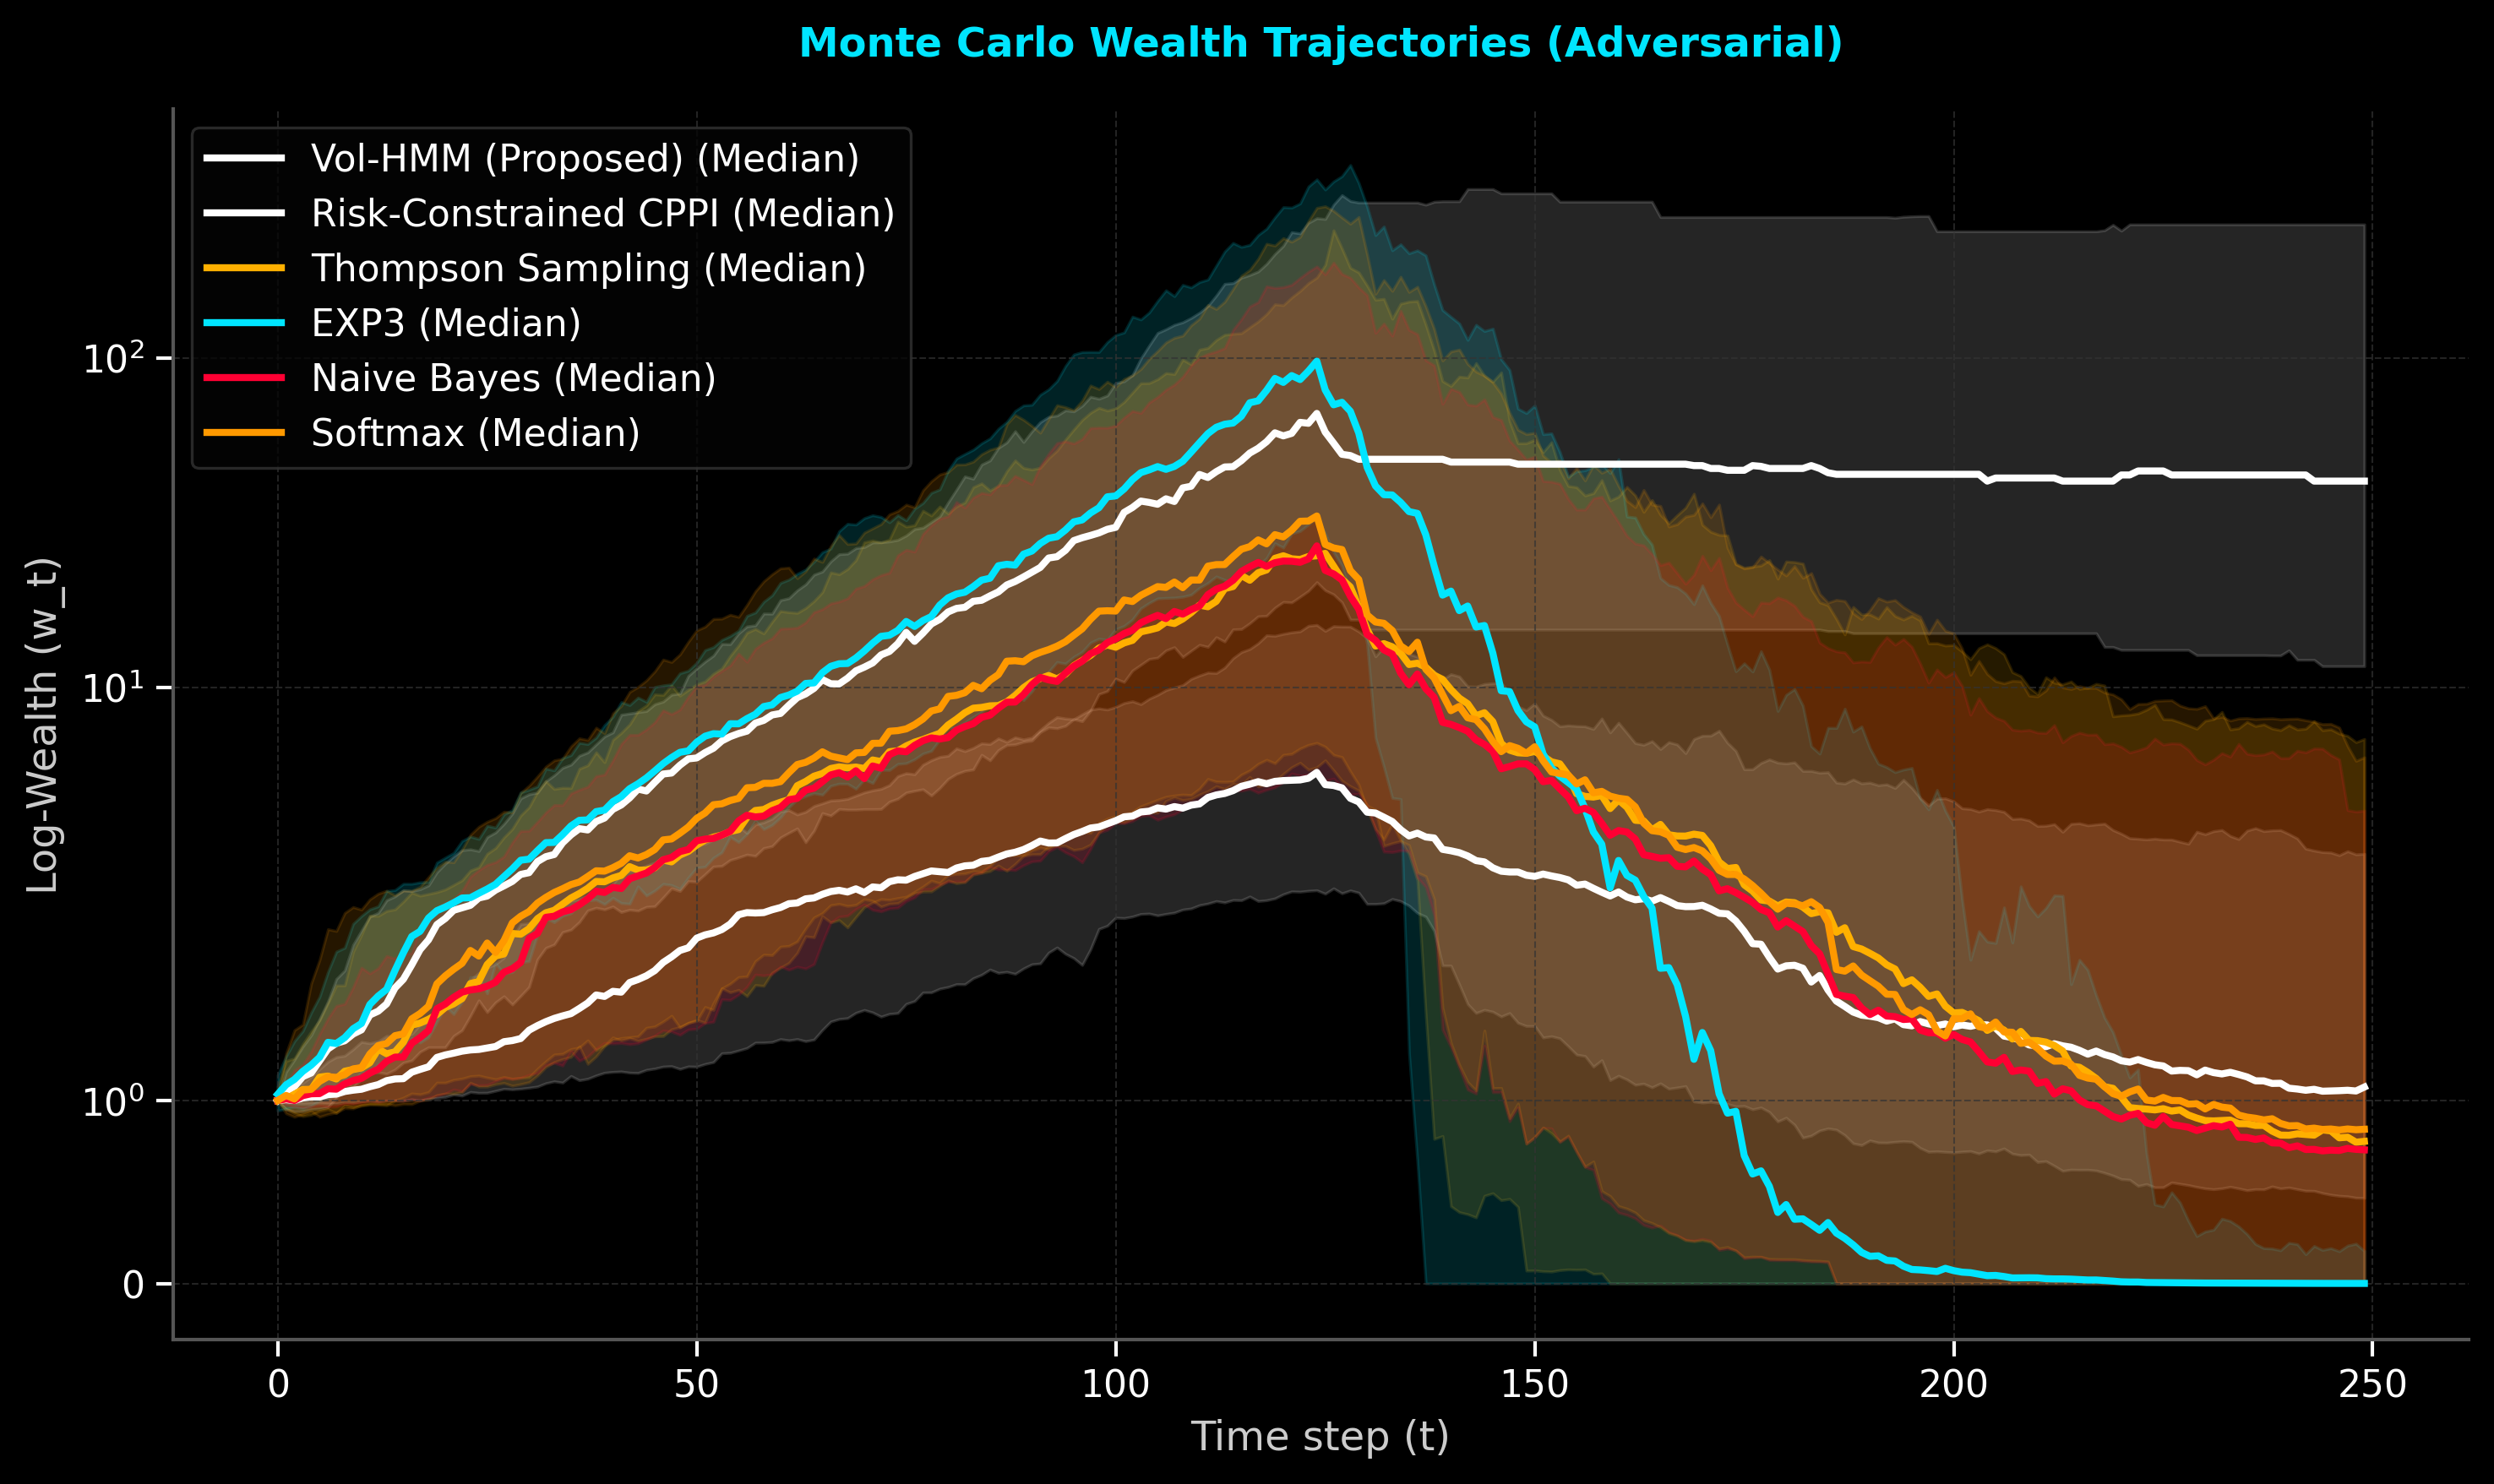
\includegraphics[width=\textwidth]{Adversarial_wealth_fan.png}\\
      {\footnotesize\color{bbdim} Monte Carlo Fan — break at $T=125$.}
    \end{column}
  \end{columns}
\end{frame}

% ── 2. MATH FRAMEWORK (02) ───────────────────────────────────
\begin{frame}{\ca{02~//}~Mathematical Framework}
  \begin{columns}[T]
    \begin{column}{0.5\textwidth}
      \ca{Filtered Probability Space}
      {\small
      \[(\Omega,\;\mathcal{F},\;\{\mathcal{F}_t\},\;\Prob)\]
      \begin{itemize}
        \item $\mathcal{F}_t = \sigma(r_1,\ldots,r_t)$ — info up to $t$.
        \item \textbf{Admissibility}: $f_t \in \mathcal{F}_{t-1}$-measurable.
        \item \textbf{Wealth}: $W_T = \prod_{t=1}^T(1+f_t r_t)$, using log-space sums for numerical stability.
      \end{itemize}
      }
    \end{column}
    \begin{column}{0.48\textwidth}
      \ca{Kelly--Breiman (SLLN)}
      \begin{block}{}
        \footnotesize
        Let $f^*=\arg\max_f \E[\ln(1+fr)]$. Then a.s.:
        \[\tfrac{1}{T}\log W_T^{(f^*)}\;\longrightarrow\;\E[\ln(1+f^*r)]\]
      \end{block}
      \vspace{0.3em}
      \ca{Sticky Prior (Proposition 3.3)}
      {\footnotesize
        After $T_0$ bull observations, posterior lag $\approx$
        $\dfrac{T_0}{2|p_1-p_0|}$ steps. For $T_0=200$, correction takes $\approx 200$ steps.
      }
    \end{column}
  \end{columns}
\end{frame}

% ── 3. AGENT HIERARCHY (03) ──────────────────────────────────
\begin{frame}{\ca{03~//}~Agent Hierarchy}
  \begin{columns}[T]
    \begin{column}{0.5\textwidth}
      \ca{Baselines}
      {\small
      \begin{itemize}
        \item \textbf{Kelly Oracle}~— Know true $\mu_t, \sigma_t$.
        \item \textbf{Naive Bayes Kelly}~— Posterior mean $\hat p$.
        \item \textbf{Thompson Sampling}~— Samples $\tilde p\sim\text{Beta}(\alpha,\beta)$.
        \item \textbf{UCB / Softmax}~— Exploration-exploitation.
        \item \textbf{EXP3 (frac)}~— Adversarial weighting.
      \end{itemize}
      }
    \end{column}
    \begin{column}{0.5\textwidth}
      \cg{Proposed Methods}
      {\small
      \begin{itemize}
        \item \cg{Vol-HMM}~— 2D observation $(r_t,v_t) +$ CUSUM.
        \item \cm{Risk-Constrained CPPI}~— Safety floor.
      \end{itemize}
      }
      \vspace{0.8em}
      \ca{Synergy}
      {\small HMM handles inference; CPPI provides a hard insurance policy against tail failure.}
    \end{column}
  \end{columns}
\end{frame}

% ── 4. VOL-HMM (04) ──────────────────────────────────────────
\begin{frame}{\cg{04~//}~Proposed Method 1: Volatility-Augmented HMM}
  \begin{columns}[T]
    \begin{column}{0.55\textwidth}
      \ca{Joint Emission (log-space)}
      {\footnotesize
      \[\ln b_j(r_t,v_t)=\ln\Normal(r_t;\mu_j,\sigma_j^2)
        +\ln\mathrm{Gamma}(v_t;k_j,\theta_j)\]
      }
      \ca{CUSUM Trigger}
      {\small $S_t^-=\max(0, S_{t-1}^- - z_t - k)$. Boosting bear belief when $S_t^- > 3.0$ is detected.}
      \vspace{0.6em}
      \ca{Bet Sizing}
      {\small $f_t = P(\text{bull} \mid \mathcal{F}_t)\cdot f^*_\text{bull}$. Cap: $f_t\in[0, 0.5]$.}
    \end{column}
    \begin{column}{0.4\textwidth}
      \ca{Detection Lag (Table 5.3)}
      \begin{center}
      \small
      \begin{tabular}{ccc}
        \toprule
        $A_{ii}$ & Lag & Ruin \\
        \midrule
        0.99 & 14.3 & 32\% \\
        \cg{0.95} & \cg{1.9} & \cg{0\%} \\
        \bottomrule
      \end{tabular}
      \end{center}
      \vspace{0.4em}
      \ca{Benefit:} \cg{87\%} faster detection of regime breaks.
    \end{column}
  \end{columns}
\end{frame}

% ── 5. CPPI (05) ─────────────────────────────────────────────
\begin{frame}{05 // Proposed Method 2: Risk-Constrained CPPI}
  \begin{columns}[T]
    \begin{column}{0.5\textwidth}
      \ca{The Risk Floor}
      {\small
      \begin{align*}
        F_t &= (1-D_{\max})\,\bar{W}_t,\quad \bar{W}_t=\max_{s\leq t}W_s\\
        \lambda_t &= \min(1,\; m \cdot C_t/W_t)
      \end{align*}
      }
      \ca{Discrete-time Logic}
      {\footnotesize
      If $m\cdot|r_{\min}|\leq 1$, then $W_{t+1}\geq F_t$. Student-$t_3$ returns violate this 25\% per step in bear markets, but $N=100$ sims show no empirical ruin.
      }
    \end{column}
    \begin{column}{0.45\textwidth}
      \centering
      \begin{tikzpicture}[scale=0.8]
        \draw[bbdim,->] (0,0) -- (4,0) node[right]{\tiny DD\%};
        \draw[bbdim,->] (0,0) -- (0,2.5) node[above]{\tiny $\lambda$};
        \draw[bbmagenta,thick] (0,2.4) -- (4,0);
        \node[bbdim,below,font=\tiny] at (0,0) {0\%};
        \node[bbdim,below,font=\tiny] at (4,0) {20\%};
      \end{tikzpicture}\\
      {\footnotesize\color{bbdim} Leverage $\lambda \to 0$ as drawdown $\to$ 20\%.}
    \end{column}
  \end{columns}
\end{frame}

% ── 6. ADVERSARIAL RESULTS (06) ───────────────────────────────
\begin{frame}{06 // Results: Adversarial Structural Break}
  \begin{columns}[T]
    \begin{column}{0.45\textwidth}
      \ca{Ruin Risk ($N=100$)}
      \begin{center}
      \small
      \begin{tabular}{lc}
        \toprule
        Agent & Ruin \\
        \midrule
        EXP3 ($f=0.5$) & 43\% \\
        Thompson & 16\% \\
        Naive Bayes & 12\% \\
        \cg{Vol-HMM} & \cg{3\%} \\
        \cm{CPPI}    & \cm{0\%} \\
        \bottomrule
      \end{tabular}
      \end{center}
      \vspace{0.5em}
      \ca{Median Terminal Wealth}
      \begin{itemize}
        \item \cg{Vol-HMM}: $42.28\times$
        \item \cm{CPPI}: $1.07\times$ (survival price)
      \end{itemize}
    \end{column}
    \begin{column}{0.55\textwidth}
      \centering
      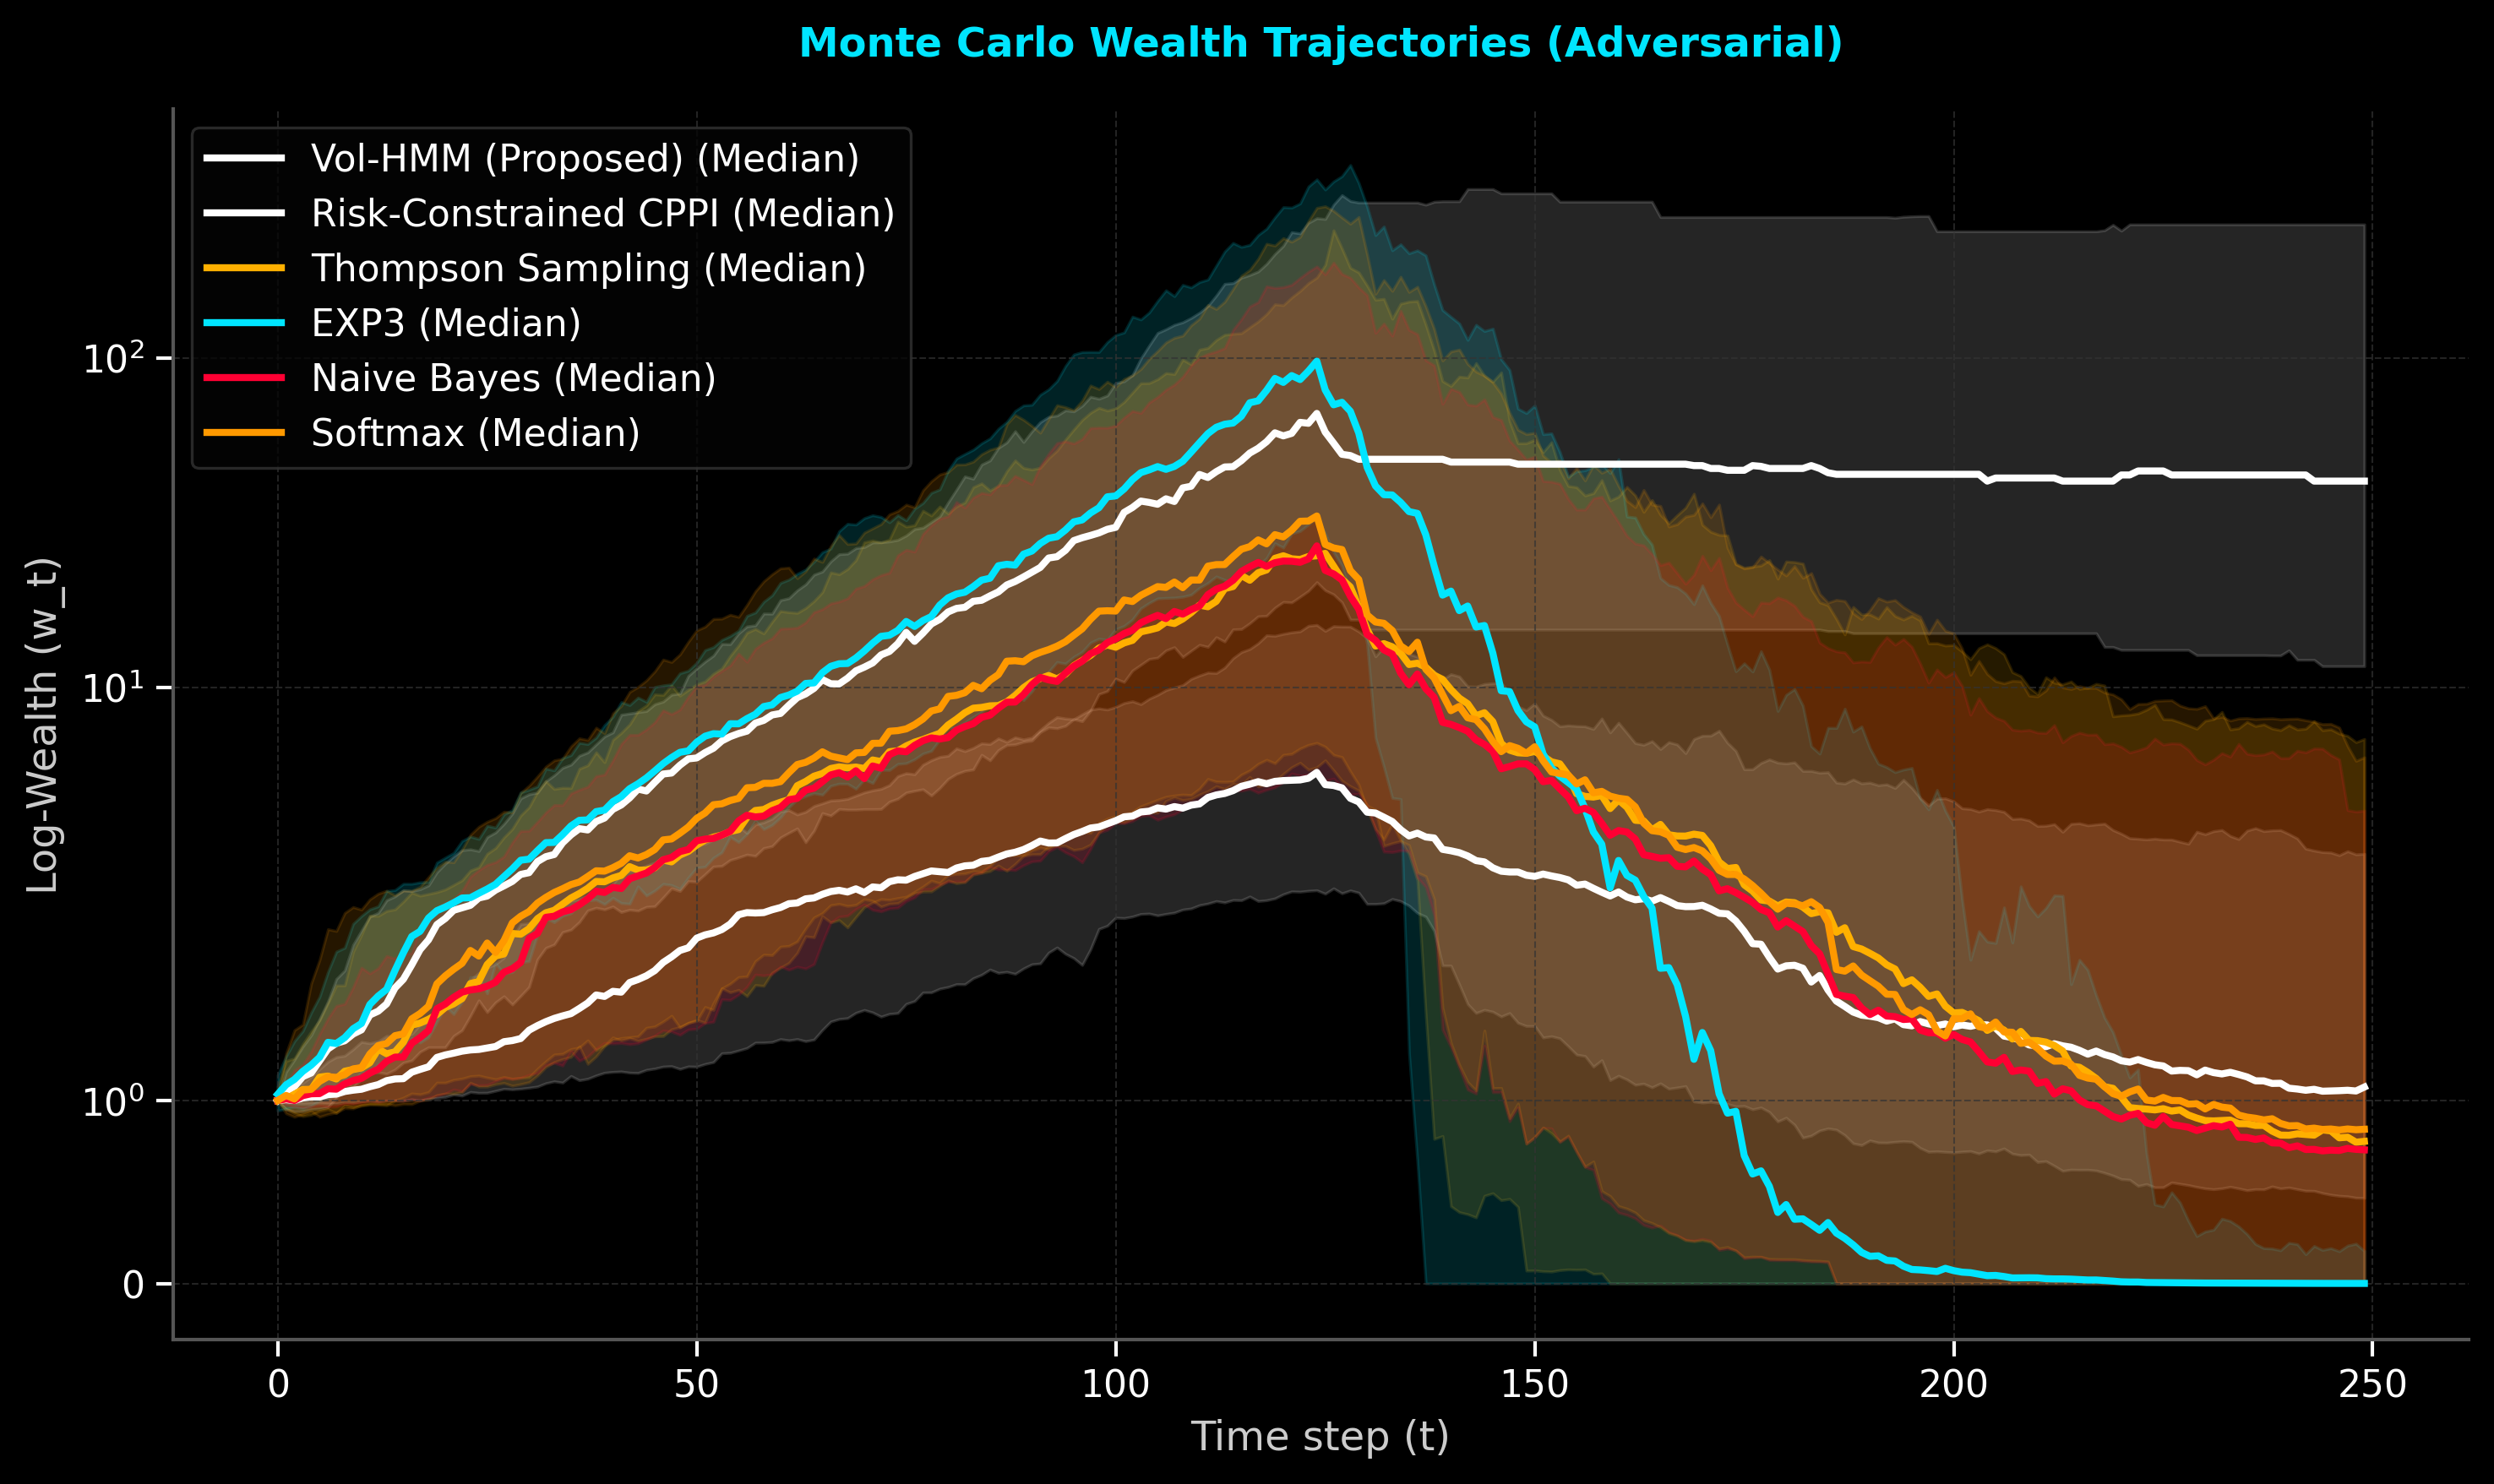
\includegraphics[width=\textwidth]{Adversarial_wealth_fan.png}\\
      {\footnotesize\color{bbdim} Divergence post-break at $T=125$.}
    \end{column}
  \end{columns}
\end{frame}

% ── 7. STATIONARY & DRIFT (07) ───────────────────────────────
\begin{frame}{\ca{07~//}~Results: Stationary \& Slow Drift}
  \begin{columns}[T]
    \begin{column}{0.5\textwidth}
      \ca{Stationary Market}
      \begin{center}
      \small
      \begin{tabular}{lc}
        \toprule
        Agent & Median $W_{250}$ \\
        \midrule
        EXP3   & $7{,}944\times$ \\
        Vol-HMM & $3{,}019\times$ \\
        Thompson & $1{,}012\times$ \\
        CPPI   & $34.9\times$ \\
        \bottomrule
      \end{tabular}
      \end{center}
      \centering
      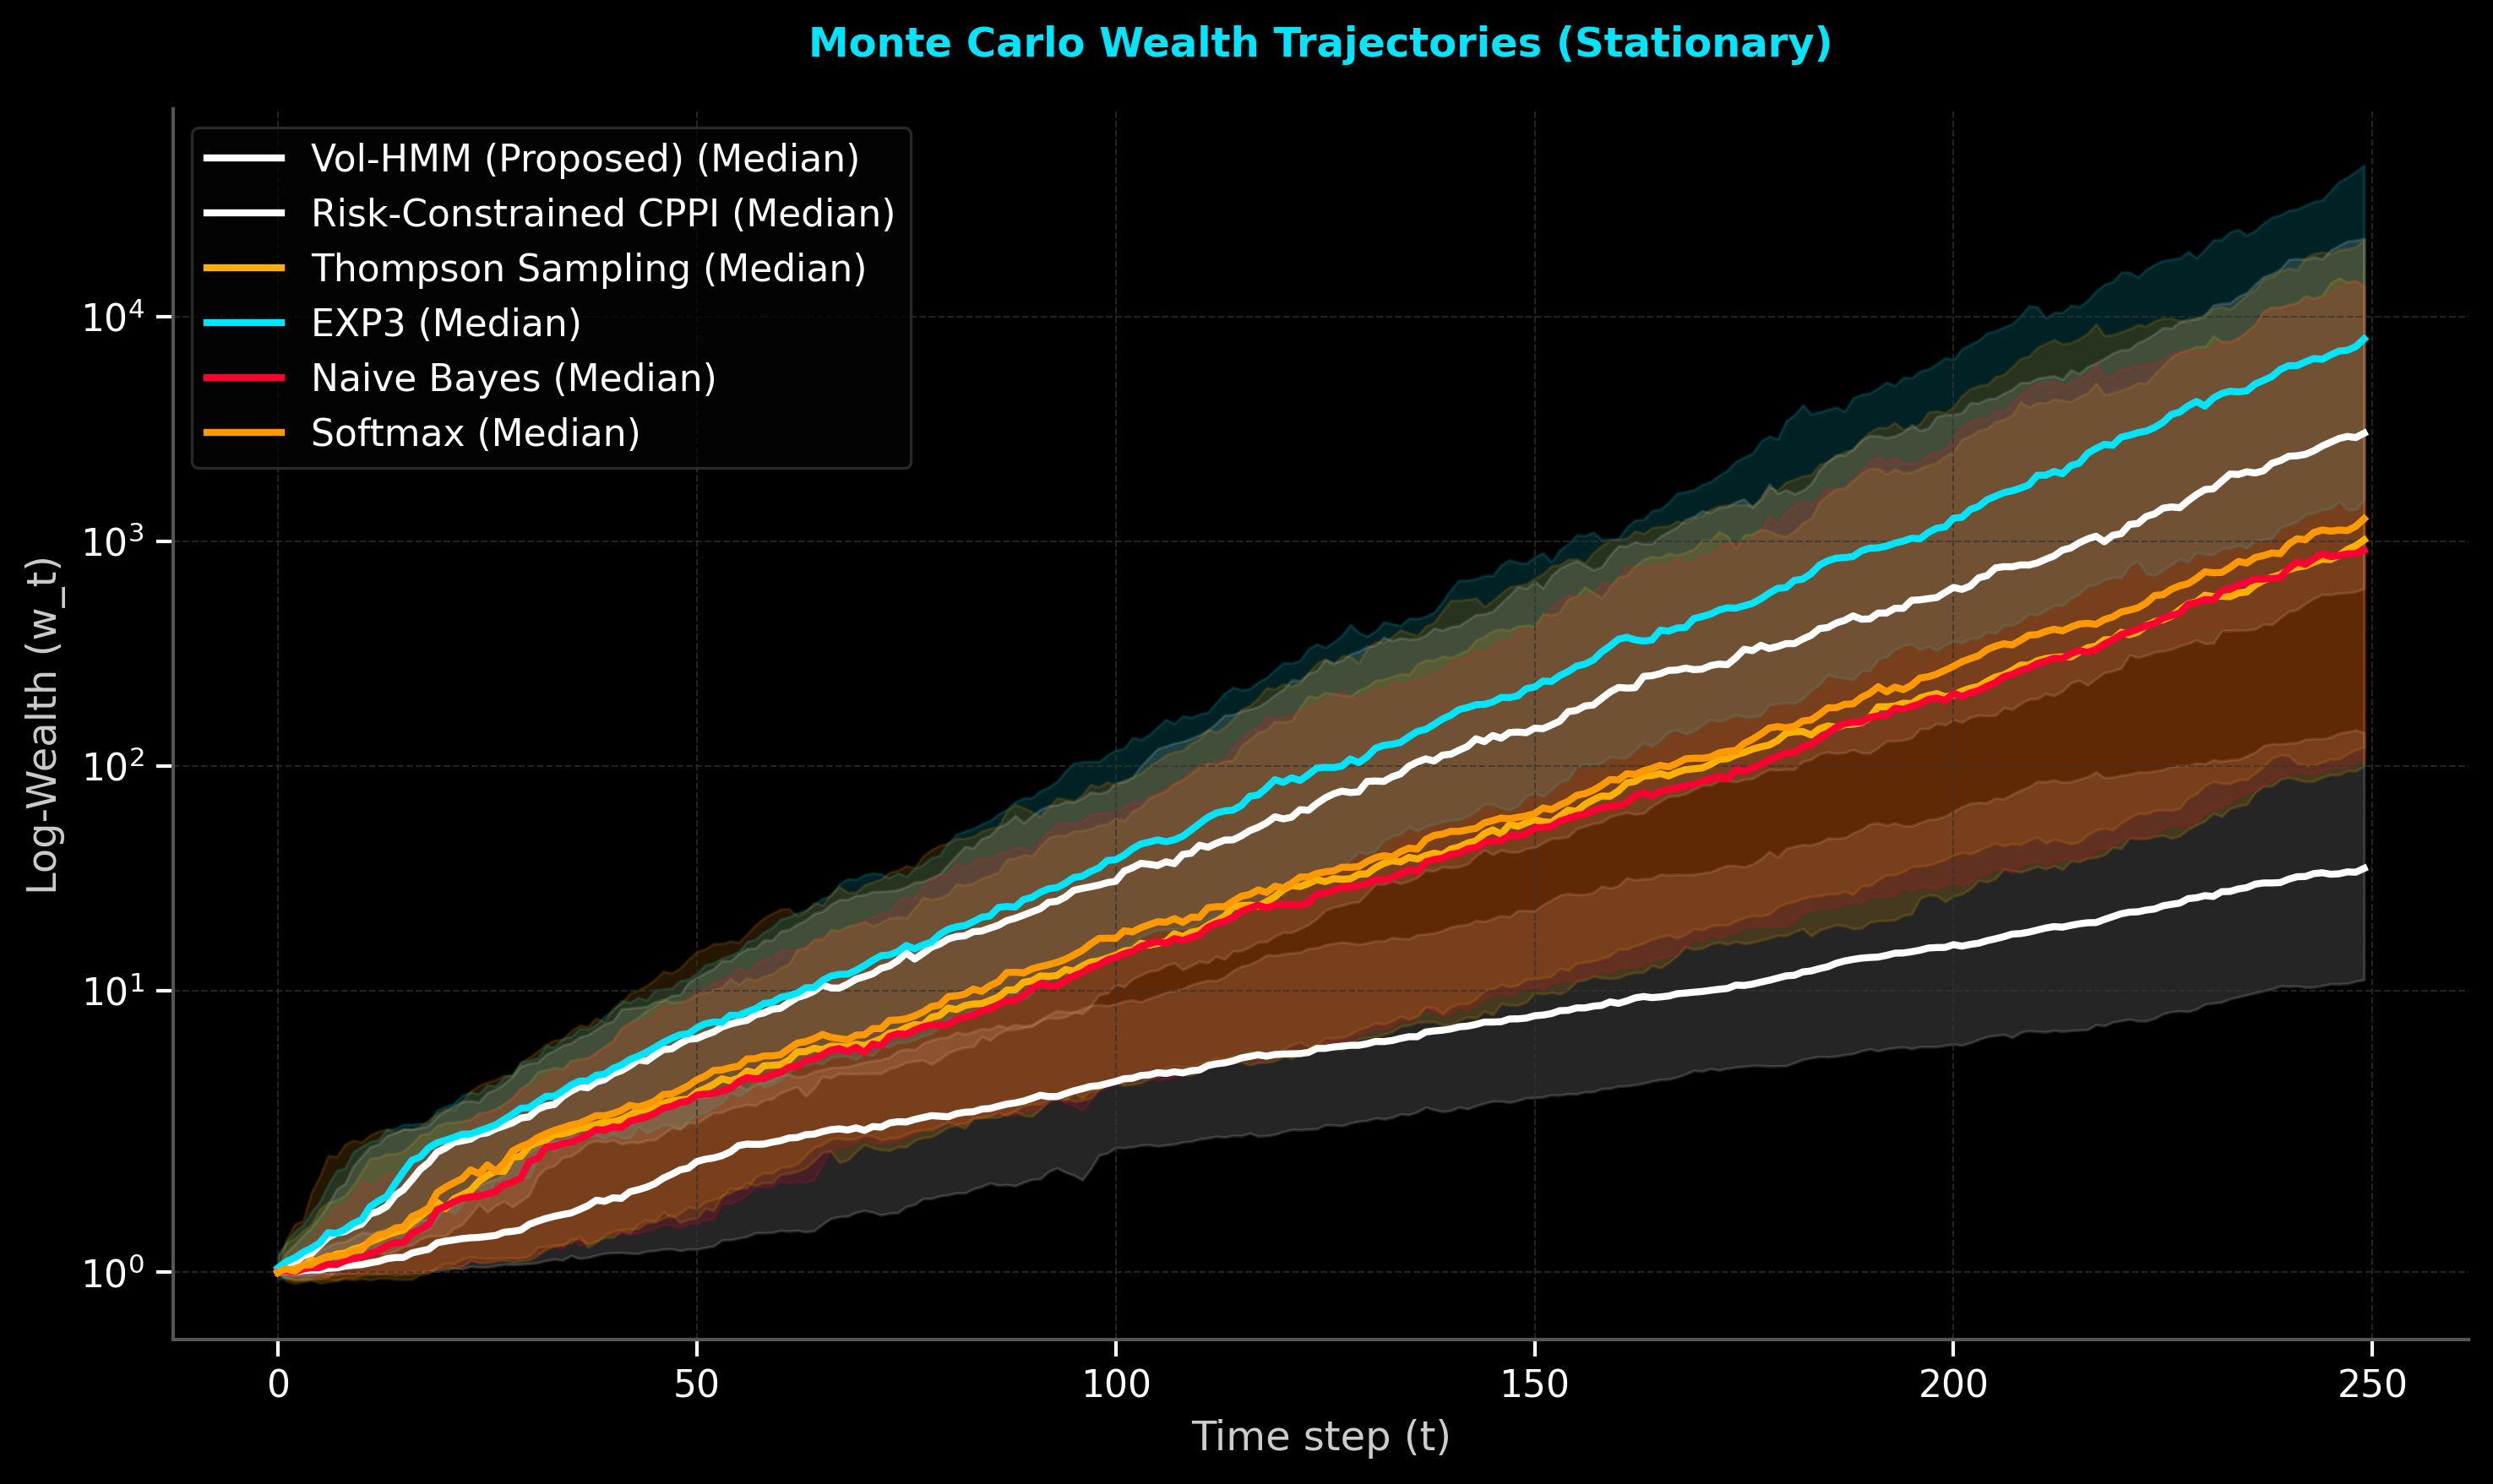
\includegraphics[width=0.85\textwidth]{Stationary_wealth_fan.png}
    \end{column}
    \begin{column}{0.5\textwidth}
      \ca{Slow Gaussian Drift}
      {\footnotesize Vol-HMM deleverages early on rising volatility, reducing regret vs Bayesian baselines.}
      \centering
      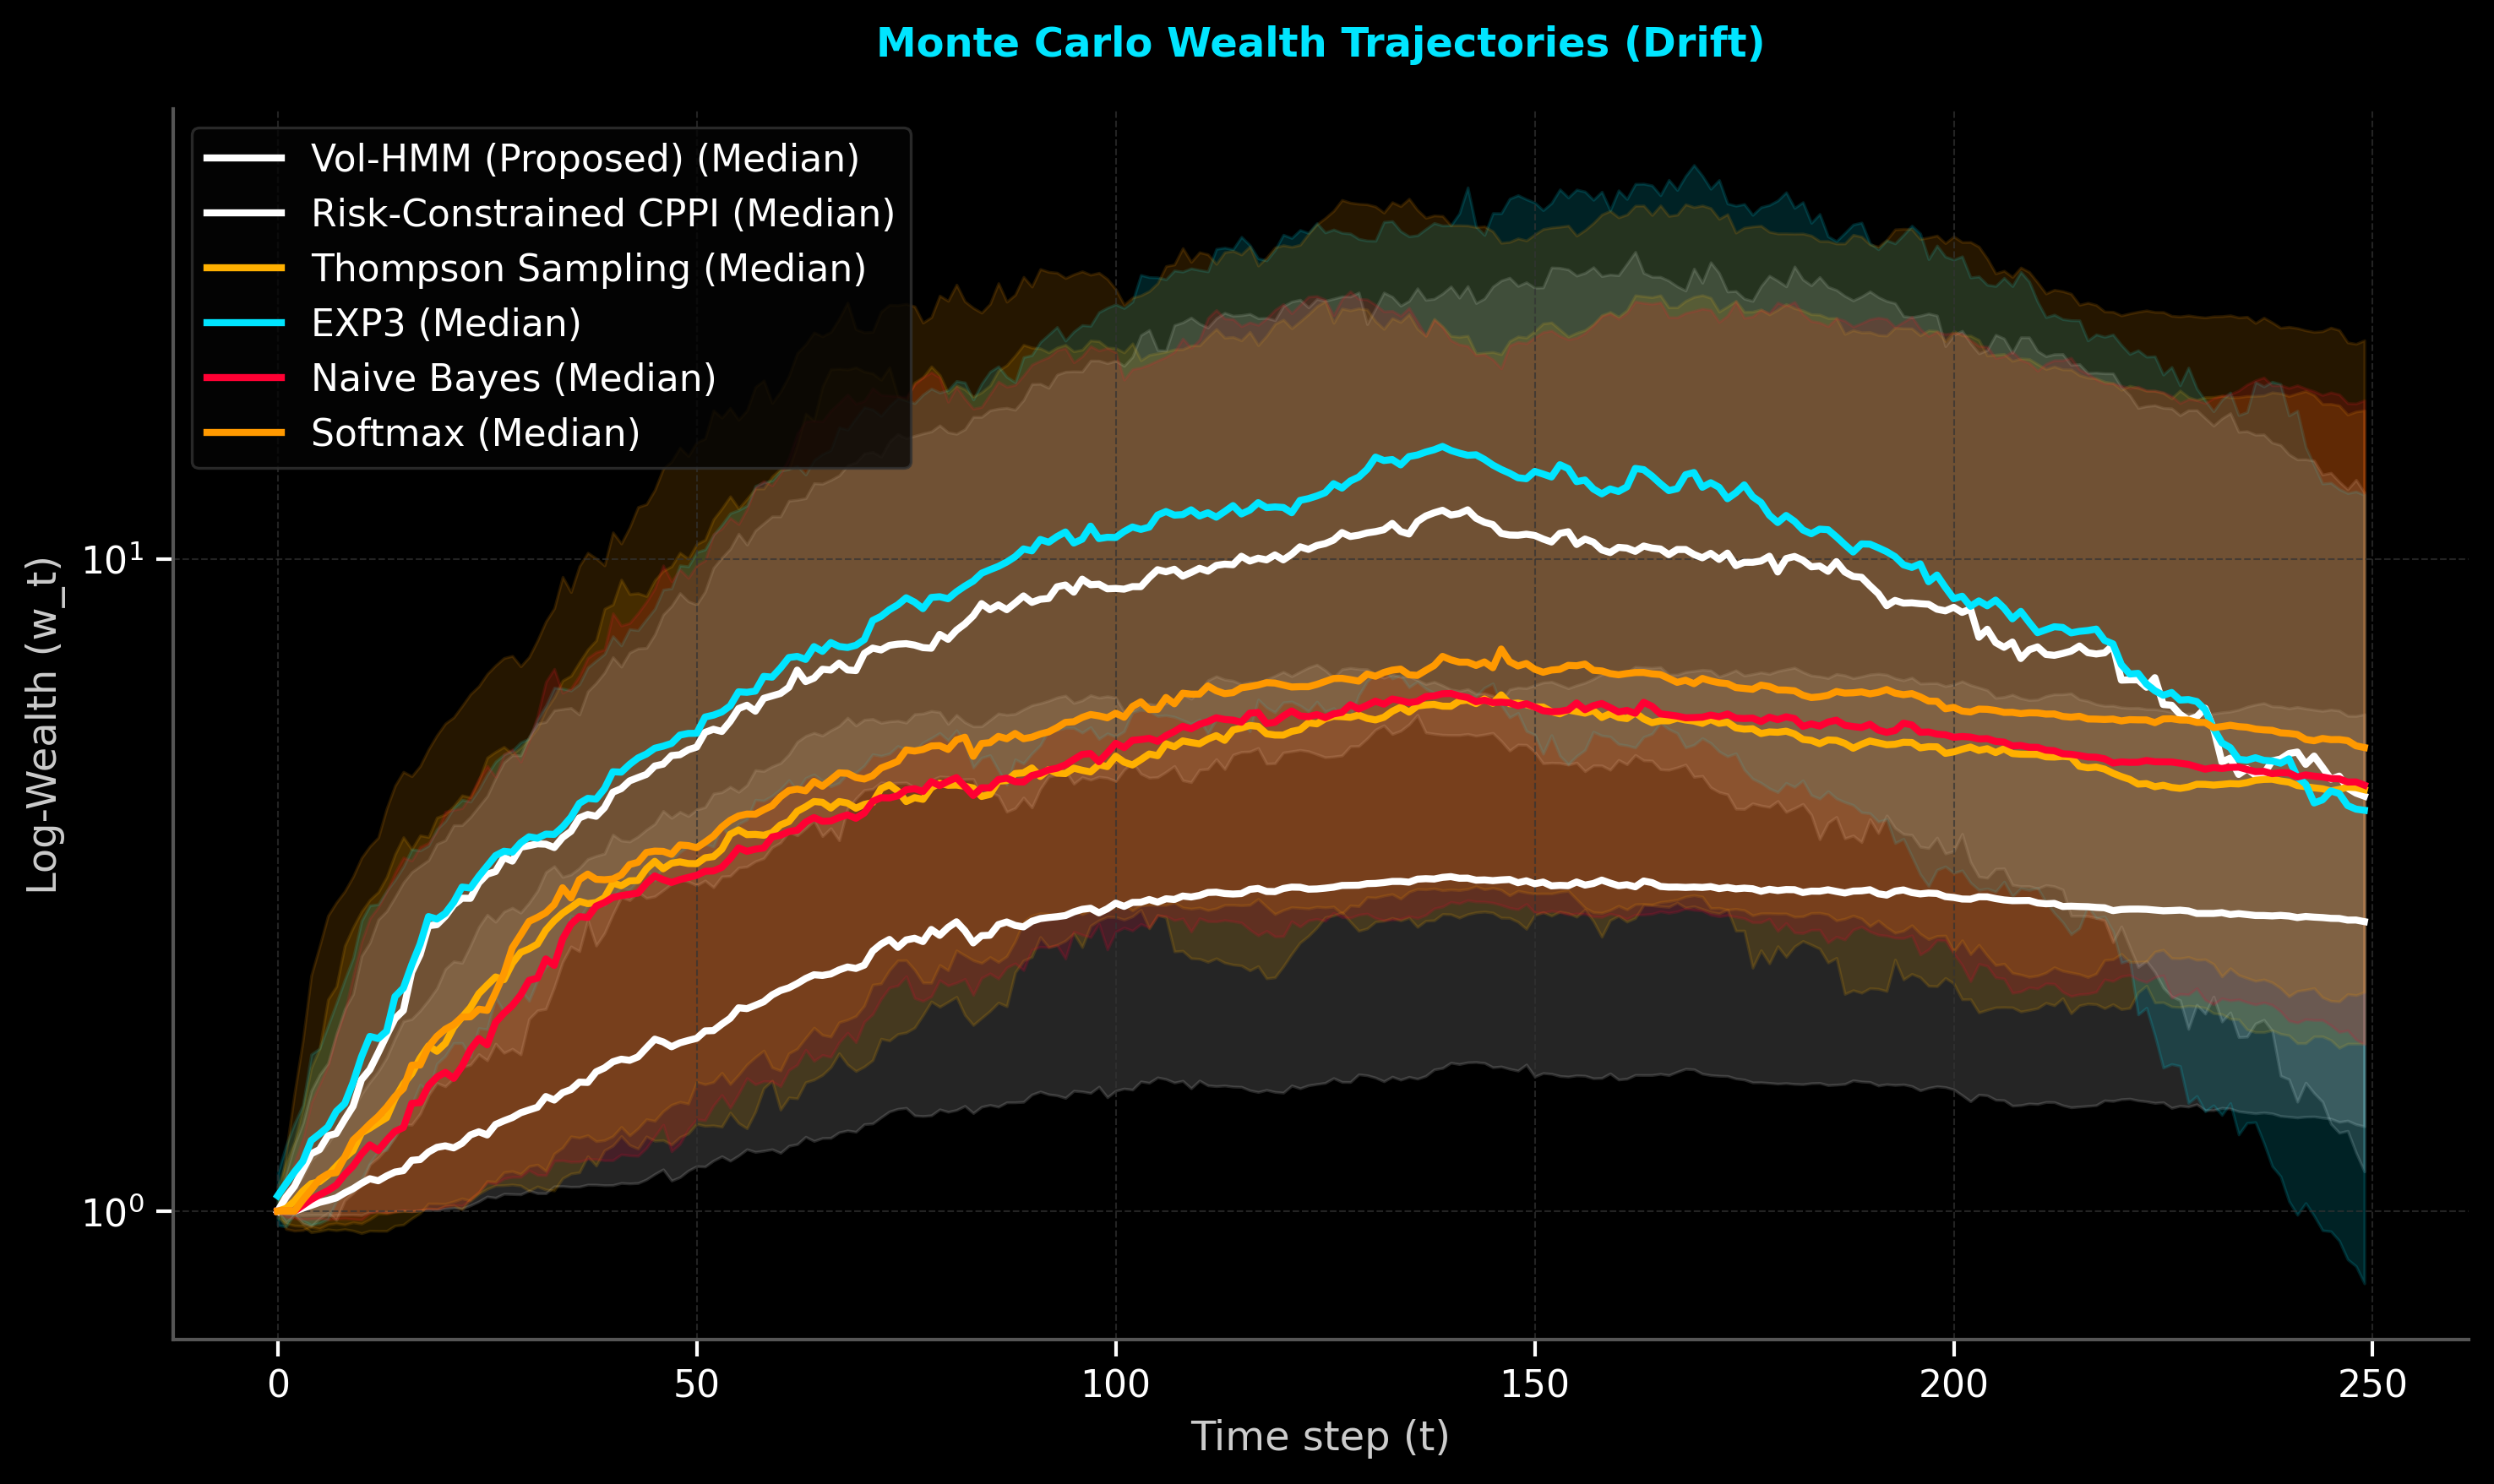
\includegraphics[width=0.85\textwidth]{Drift_wealth_fan.png}
    \end{column}
  \end{columns}
\end{frame}

% ── 8. REGRET DYNAMICS (08) ───────────────────────────────
\begin{frame}{\ca{08~//}~Oracle Regret Dynamics}
  \begin{columns}[T]
    \begin{column}{0.5\textwidth}
      \centering
      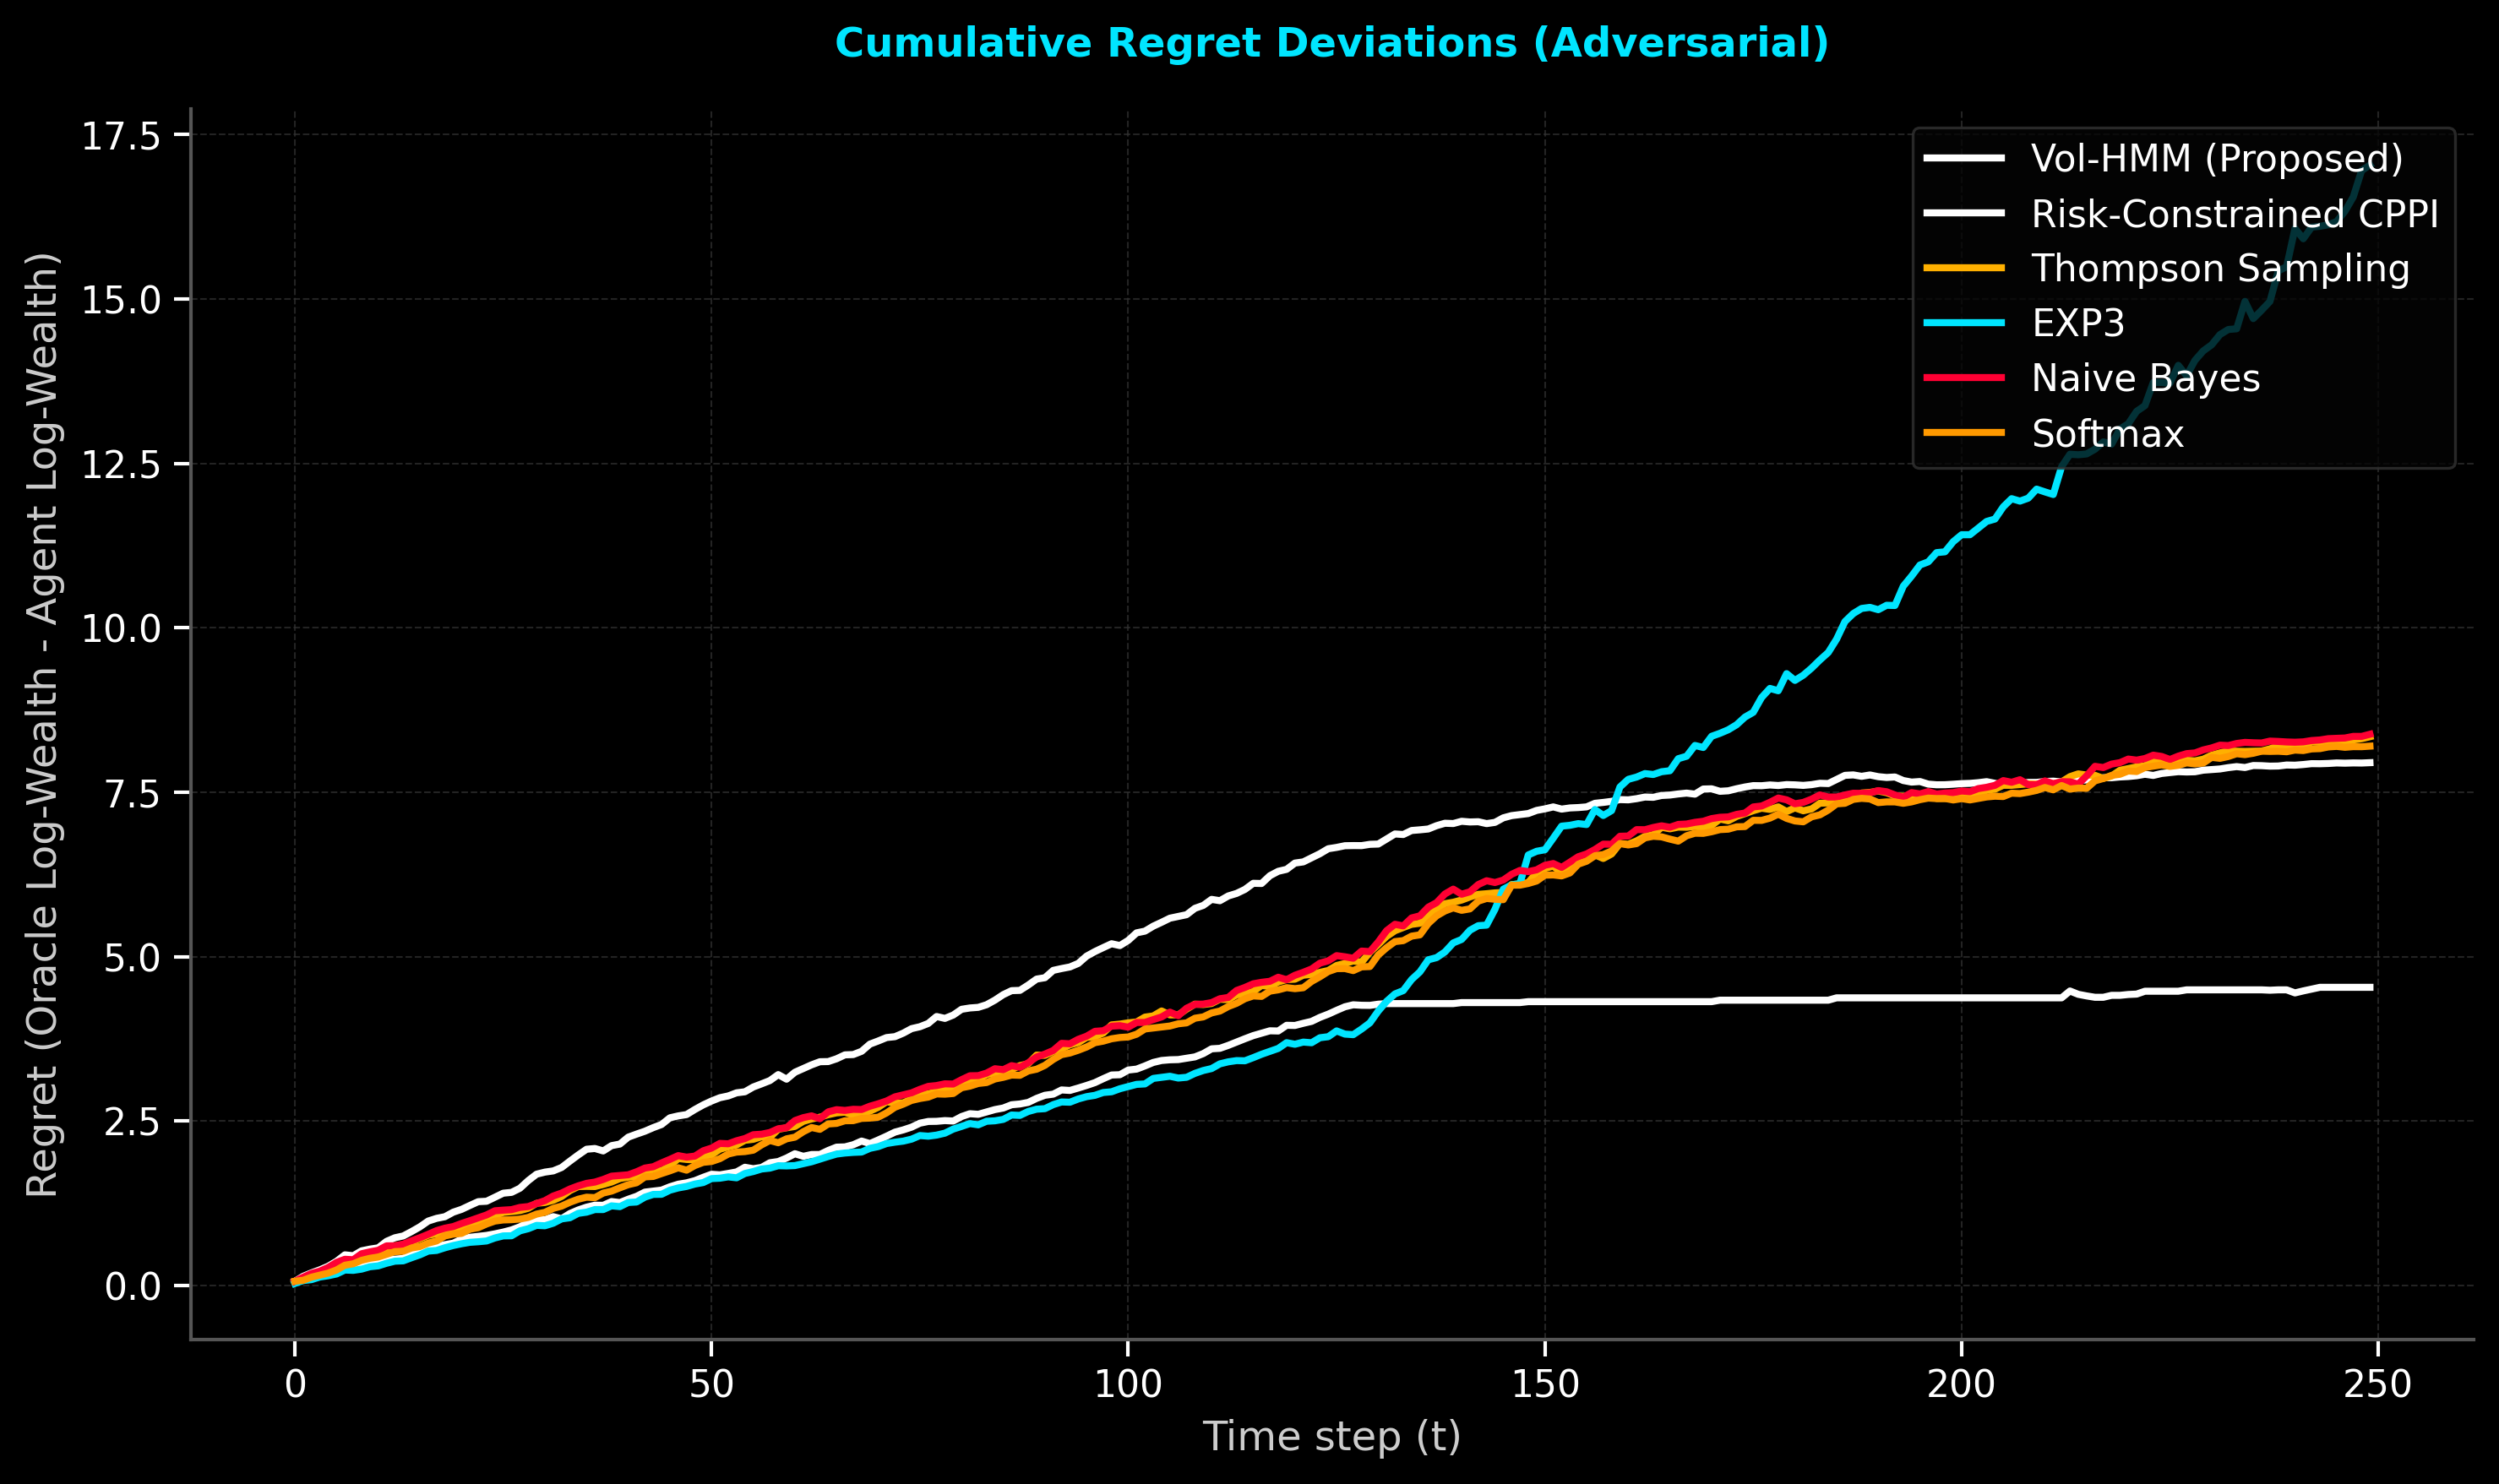
\includegraphics[width=0.9\textwidth]{Adversarial_regret_dynamics.png}\\
      {\footnotesize\ca{Adversarial}: sharp inflection at break.}
    \end{column}
    \begin{column}{0.5\textwidth}
      \centering
      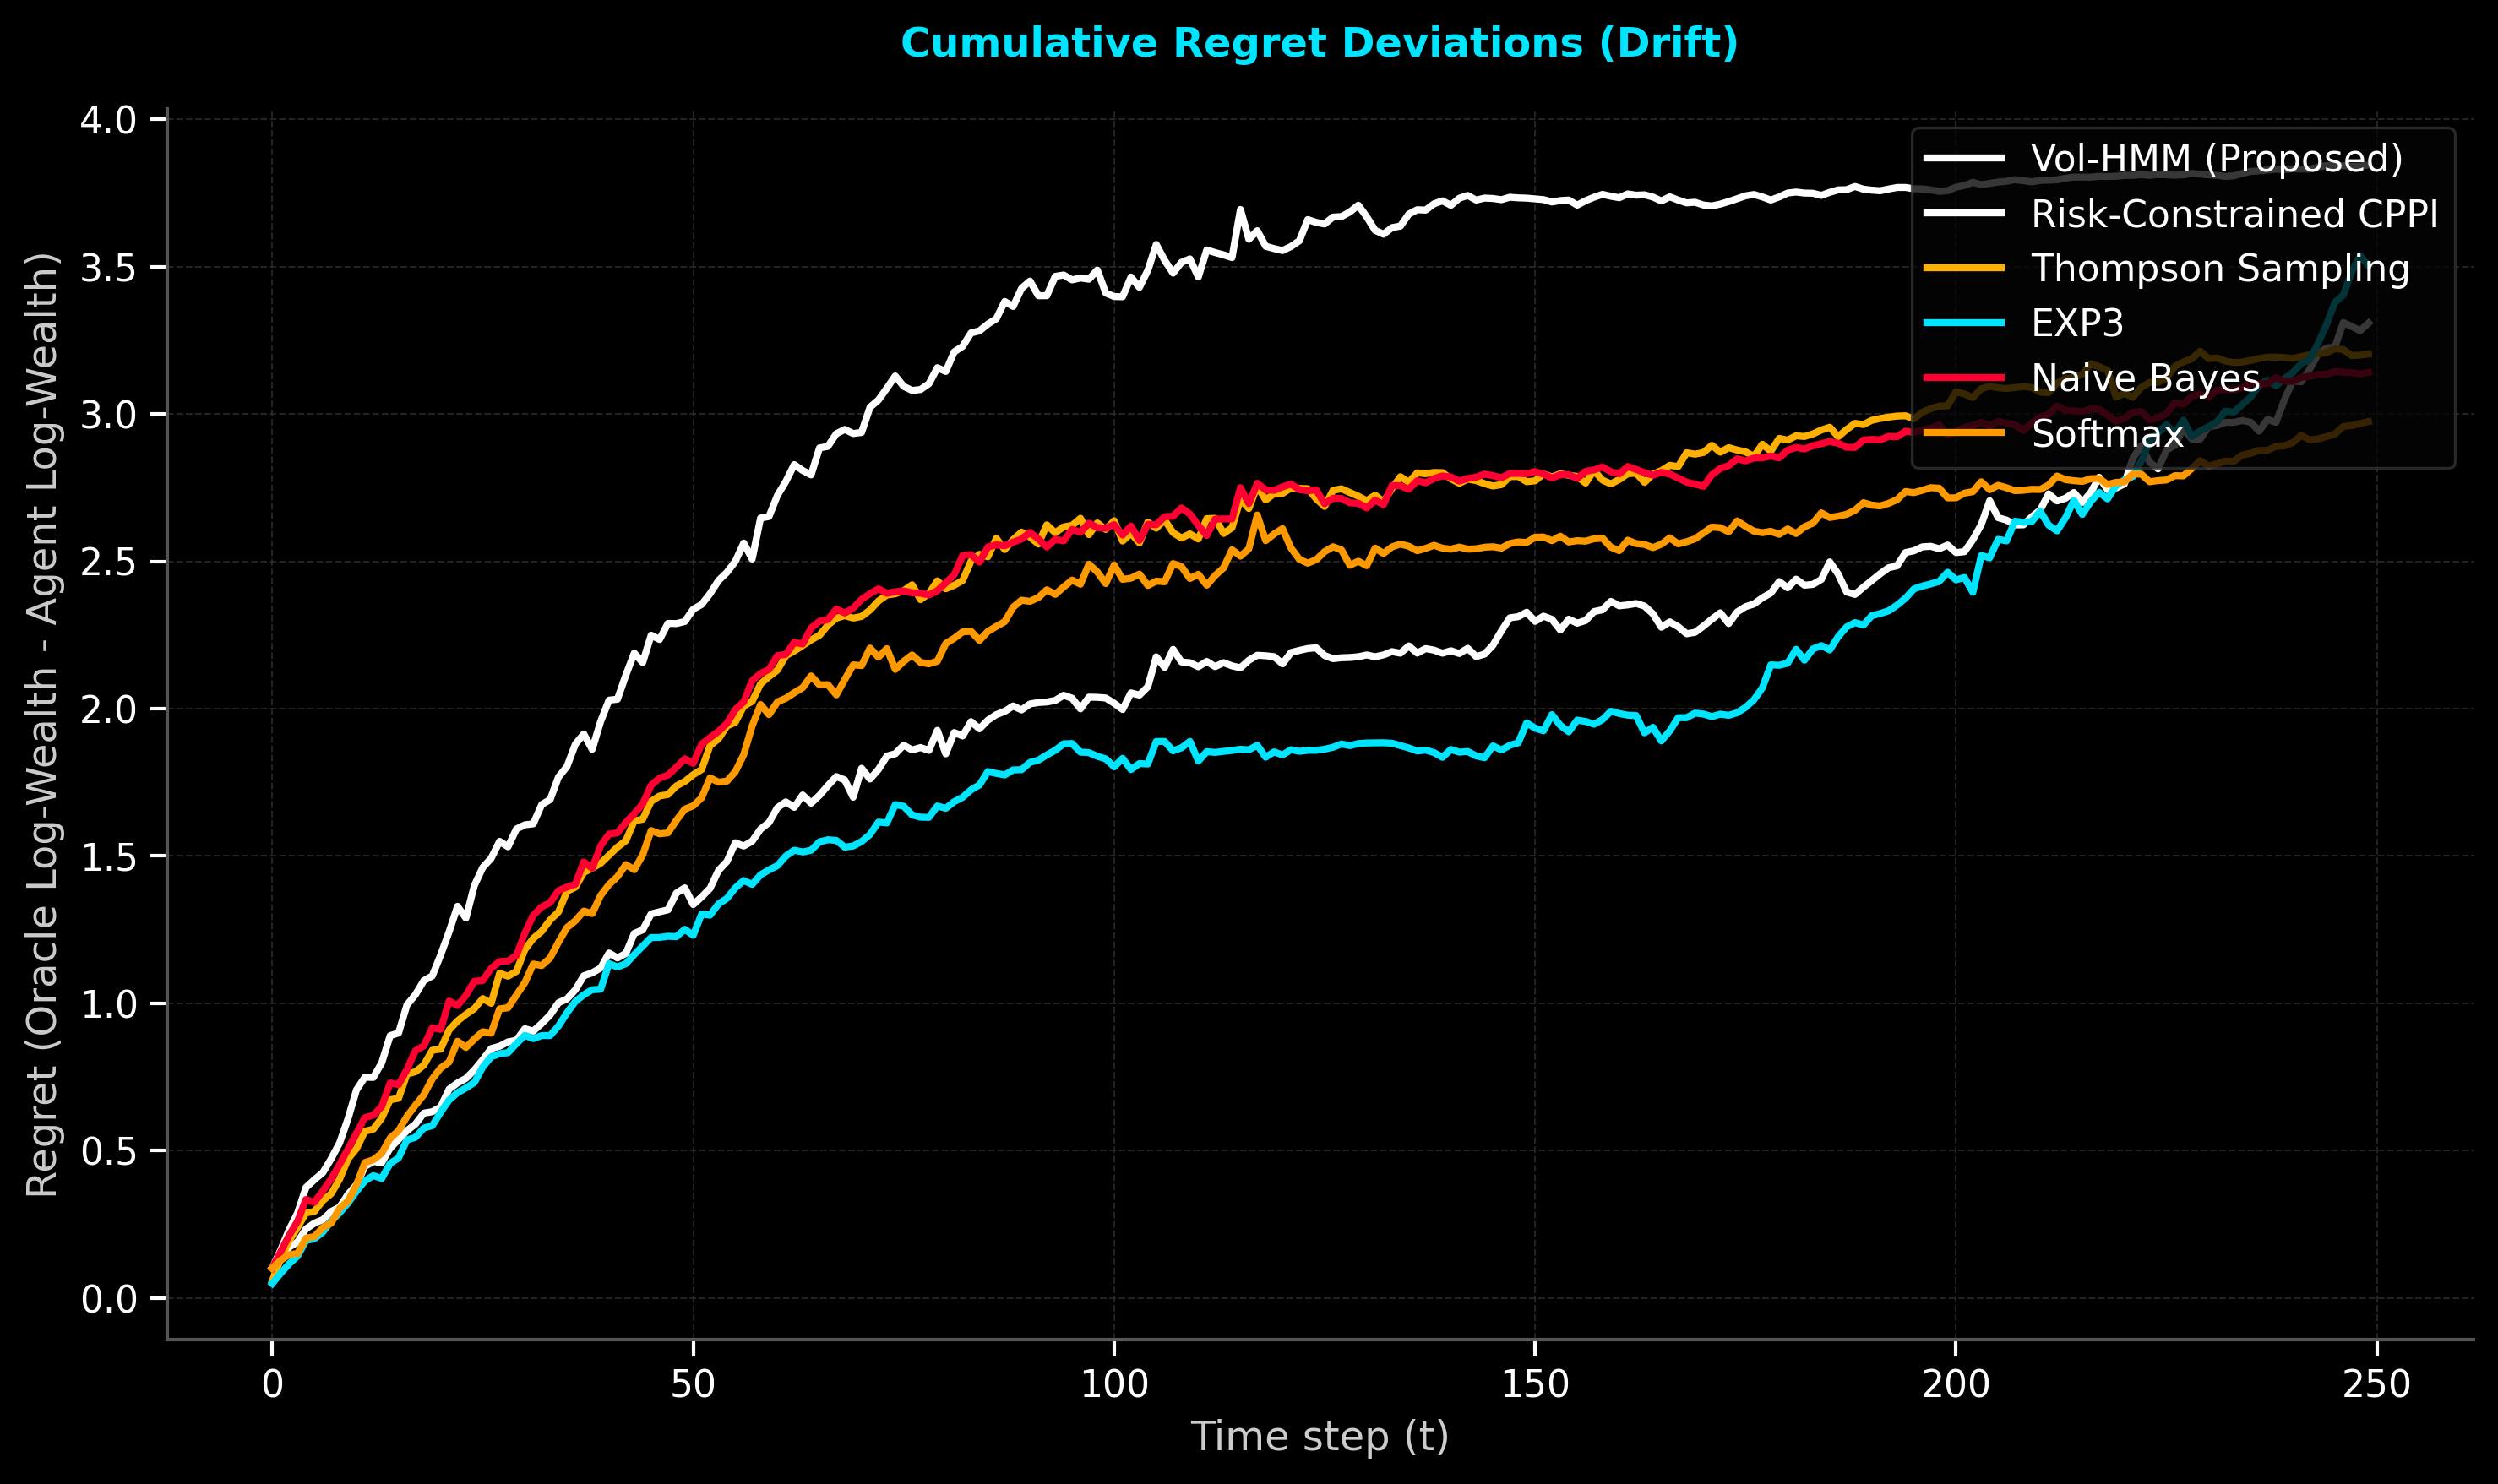
\includegraphics[width=0.9\textwidth]{Drift_regret_dynamics.png}\\
      {\footnotesize\ca{Drift}: gradual regret buildup.}
    \end{column}
  \end{columns}
  \vspace{0.4em}
  {\footnotesize Lower Regret = Better and closer to the Kelly Oracle.}
\end{frame}

% ── 9. STATISTICAL SIGNIFICANCE (09) ───────────────────────
\begin{frame}{09 // Statistical Significance}
  \begin{columns}[T]
    \begin{column}{0.48\textwidth}
      \ca{Fisher's Exact Test} (Ruin)\\[4pt]
      $H_0$: Vol-HMM and EXP3 have equal ruin rates.\\[4pt]
      \begin{center}
      \small
      \begin{tabular}{lcc}
        \toprule
         & Ruined & Survived \\
        \midrule
        EXP3    & 43 & 57 \\
        Vol-HMM & 3  & 97 \\
        \bottomrule
      \end{tabular}
      \end{center}
      \[\Rightarrow\; p < 0.001\]
      Null rejected: survival alpha is significant.
    \end{column}
    \begin{column}{0.52\textwidth}
      \centering
      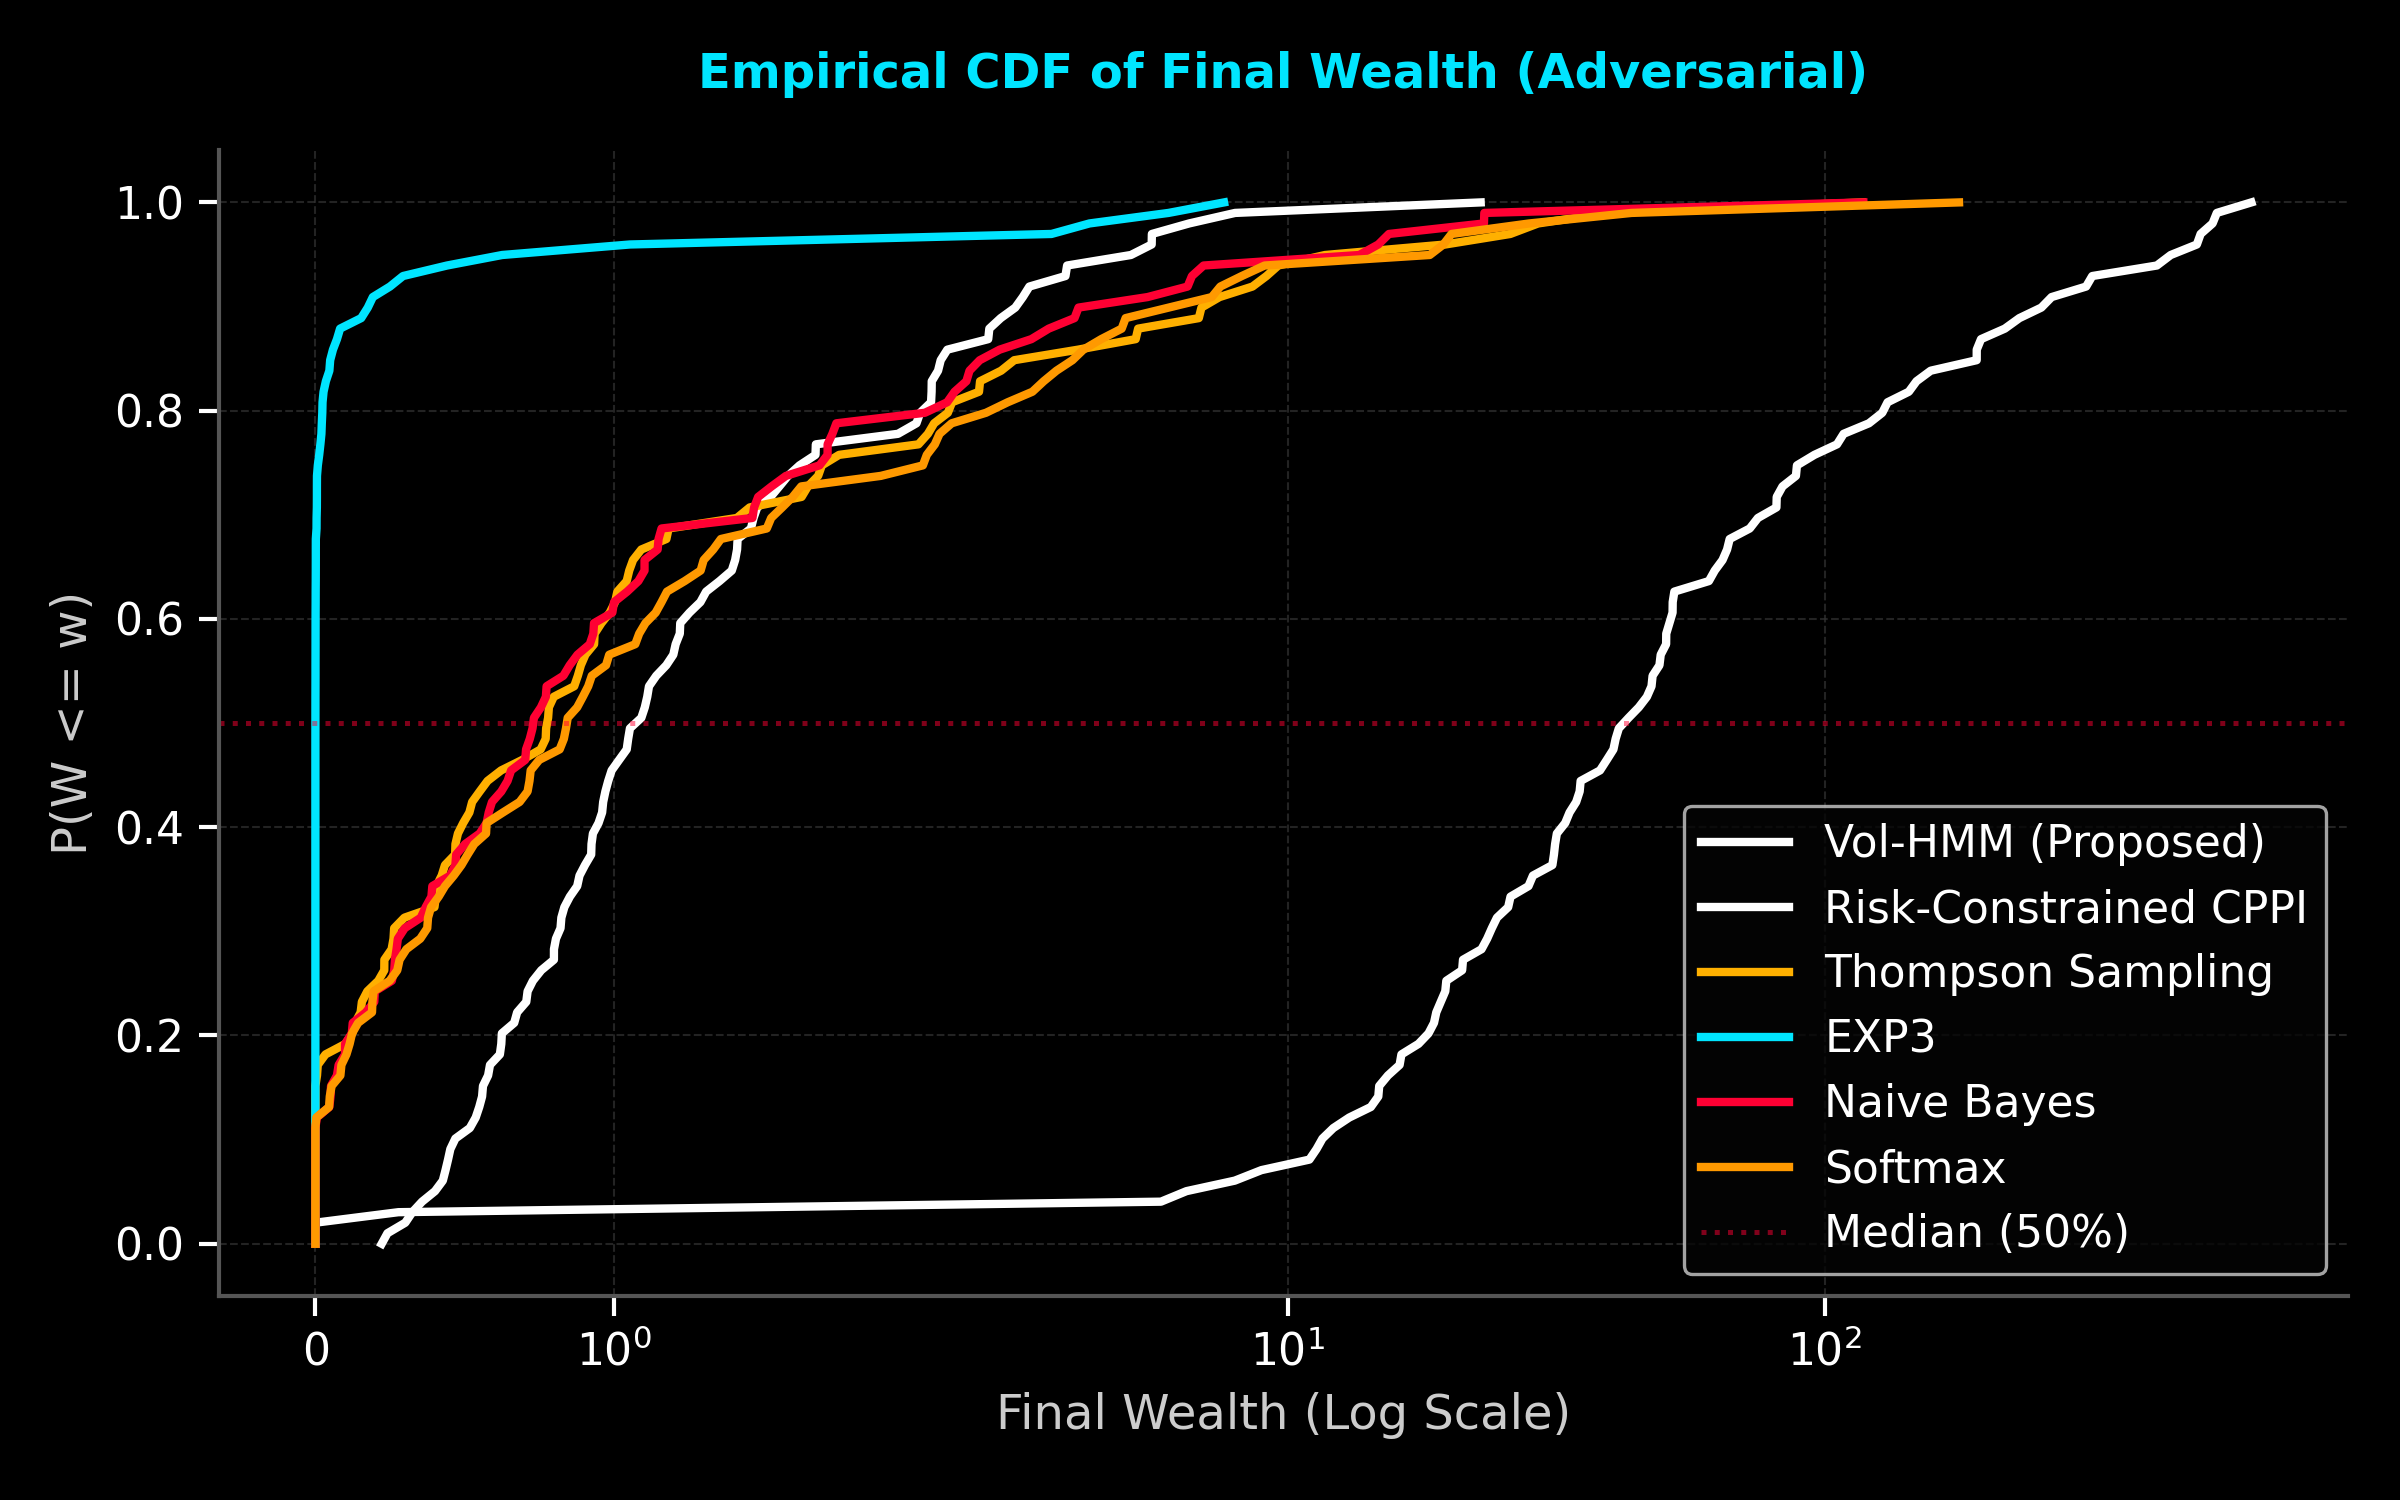
\includegraphics[width=0.9\textwidth]{Adversarial_cdf.png}\\
      {\footnotesize\color{bbdim} CDF of Terminal Wealth (Adversarial).}
    \end{column}
  \end{columns}
\end{frame}

% ── 10. HISTORICAL VALIDATION (10) ───────────────────────────
\begin{frame}{\ca{10~//}~Historical Validation: S\&P 500}
  \begin{center}
  \small
  \begin{tabular}{lcccc}
    \toprule
    Epoch & Days & Agent & Wealth & Sortino \\
    \midrule
    2008 GFC & 523 & \cg{Vol-HMM} & $0.88\times$ & $+0.45$ \\
             &     & \cm{CPPI}    & $0.80\times$ & $\mathbf{+0.82}$ \\
             &     & Buy-and-Hold  & $0.62\times$ & $-0.32$ \\
    \midrule
    2020 COVID & 251 & Vol-HMM & \multicolumn{2}{r}{Detection in $\approx$ 2 days} \\
    \midrule
    2013-19 Bull & 1,760 & CPPI & \multicolumn{2}{r}{Growth drag (survival cost)} \\
    \bottomrule
  \end{tabular}
  \end{center}
  \vspace{0.4em}
  \ca{Sortino Metric:} Using \textbf{Downside Deviation} ($\hat\sigma_\downarrow$) as the denominator. Captures actual tail risk exposure that simple volatility obscures.
\end{frame}

% ── 11. TRANSACTION COSTS (11) ───────────────────────────────
\begin{frame}{\ca{11~//}~Transaction Costs: The Net Advantage}
  \begin{columns}[T]
    \begin{column}{0.5\textwidth}
      \ca{Turnover Advantage}
      {\small
      \begin{itemize}
        \item Bayesian agents whipsaw on noisy updates.
        \item Vol-HMM rebalances only on persistent regime shifts.
        \item Annualized Fee Drag (25 bps):
          \begin{itemize}
            \item Thompson: $0.6\%$/yr
            \item \cg{Vol-HMM}: $0.15\%$/yr
          \end{itemize}
      \end{itemize}
      }
    \end{column}
    \begin{column}{0.5\textwidth}
      \centering
      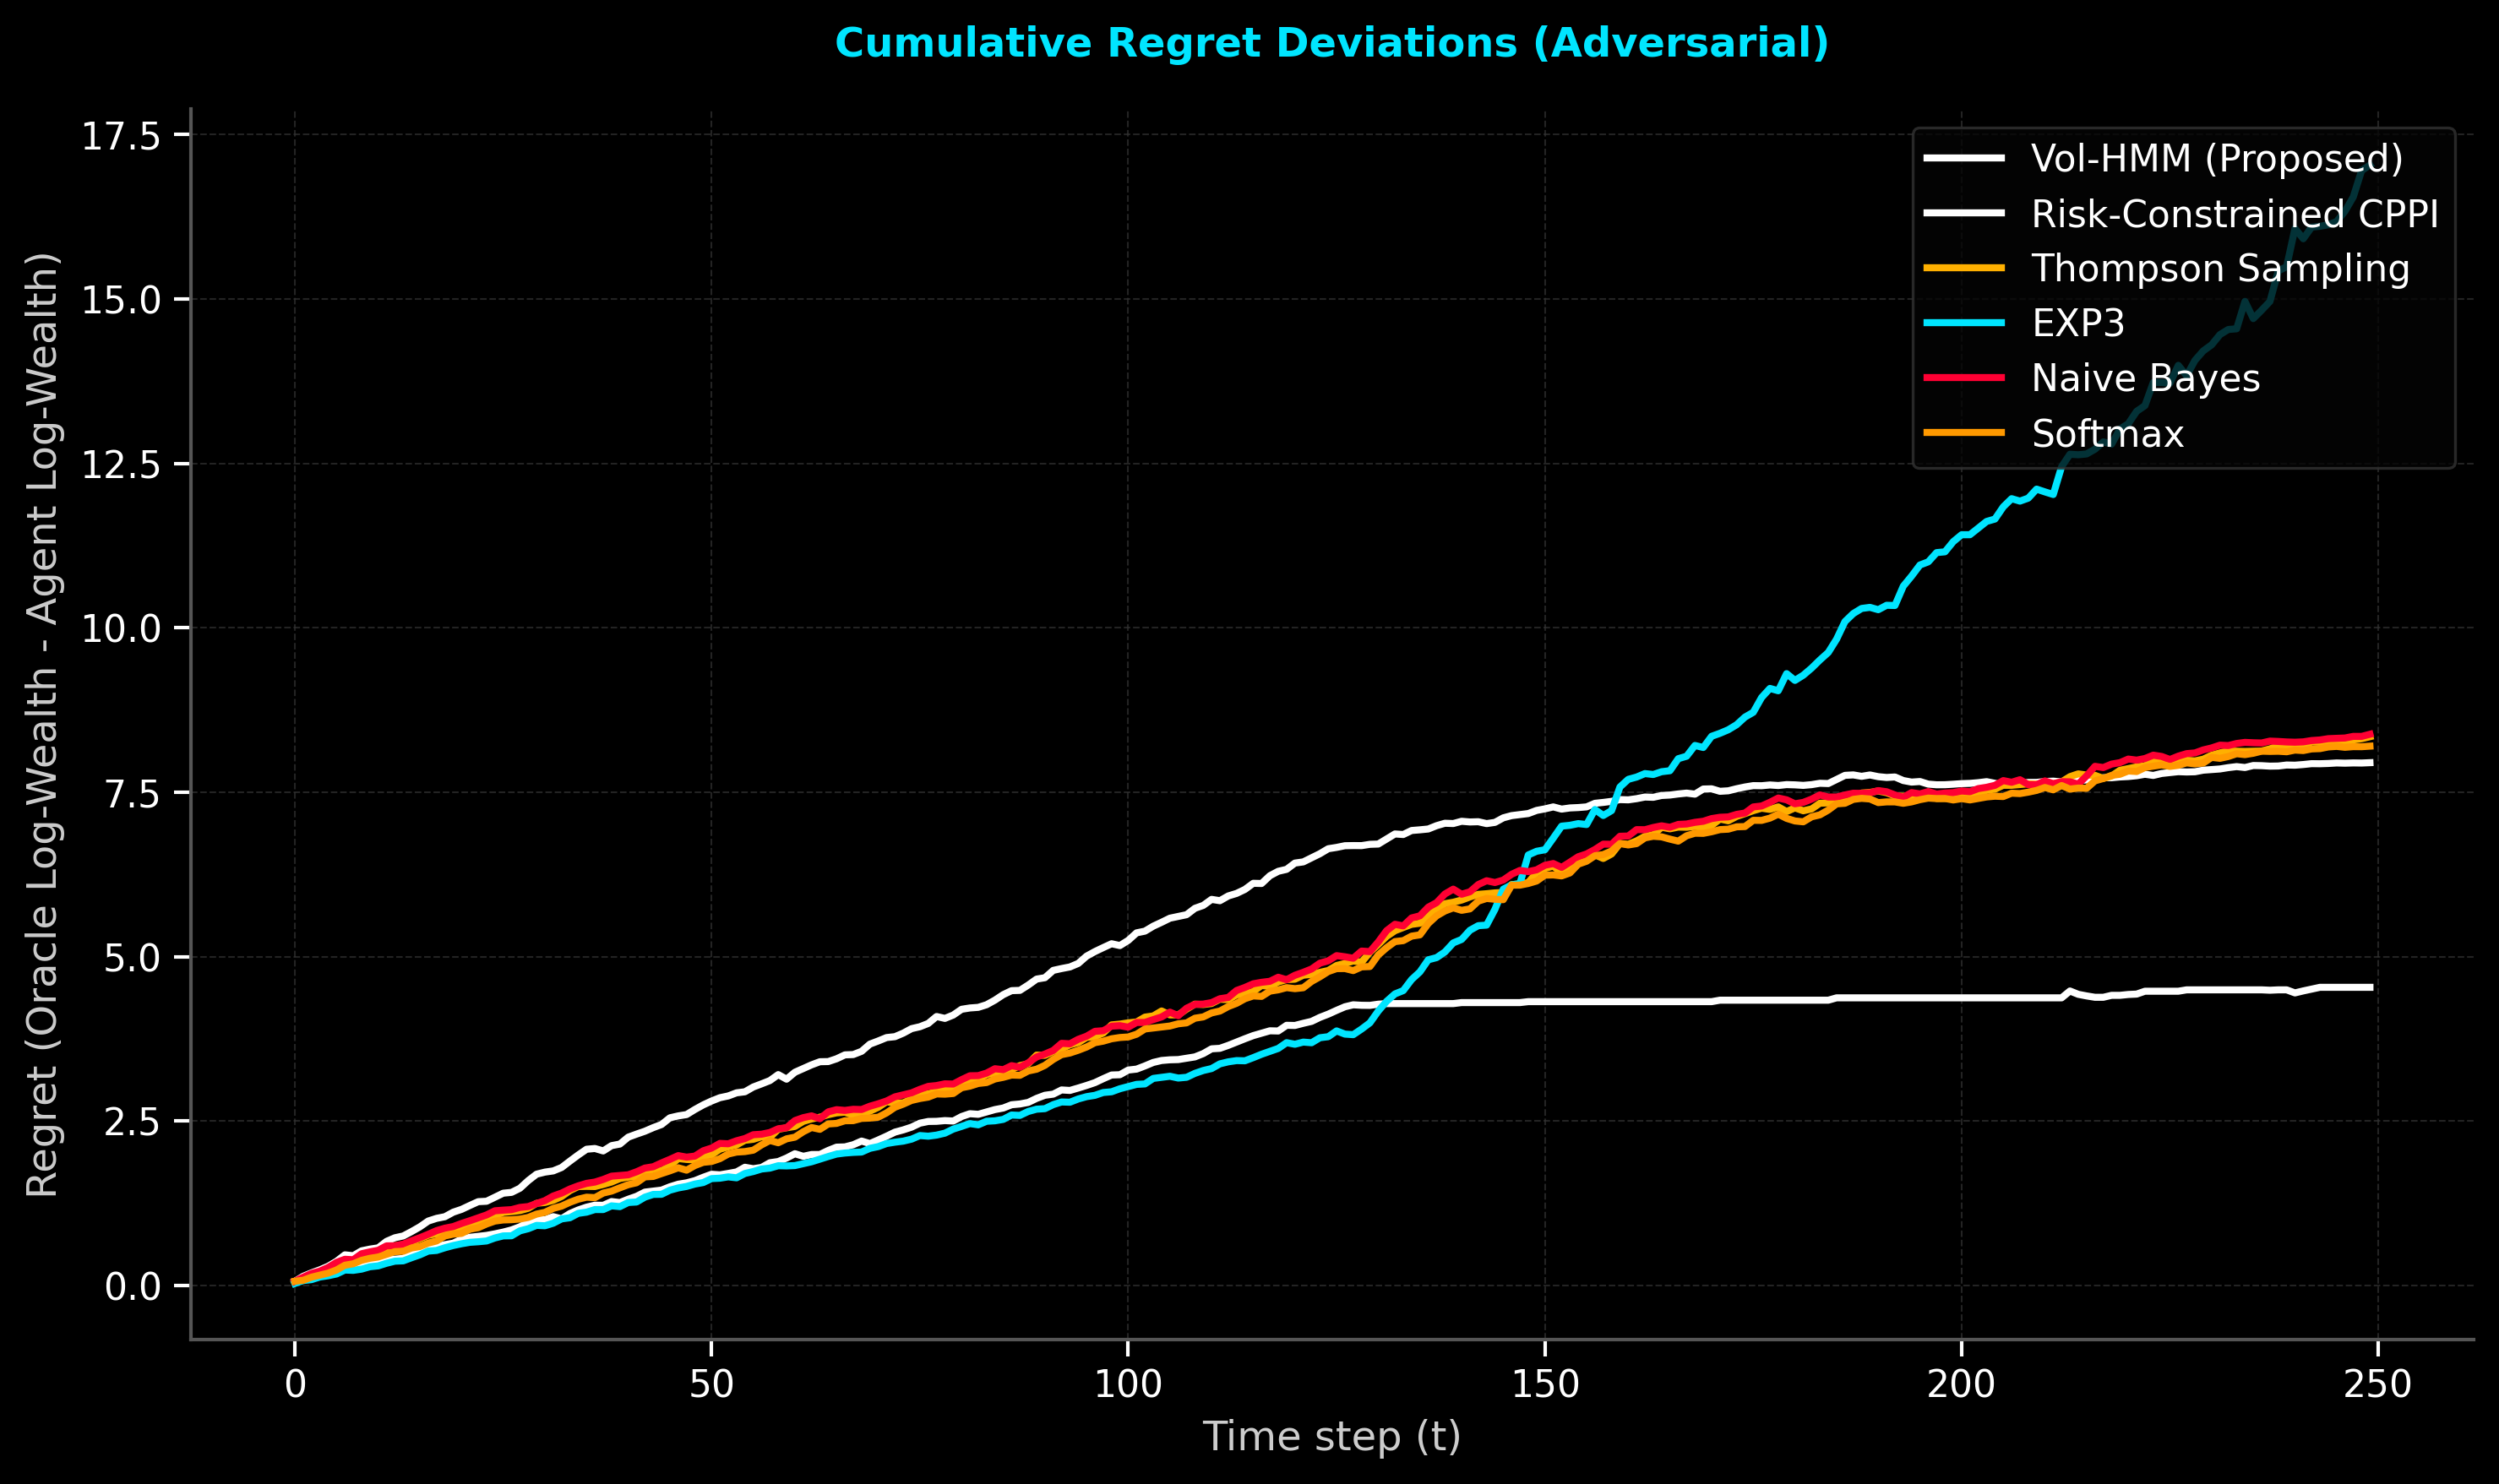
\includegraphics[width=0.95\textwidth]{Adversarial_regret_dynamics.png}\\
      {\footnotesize\color{bbdim} Regret spread increases at high friction.}
    \end{column}
  \end{columns}
\end{frame}

% ── 12. LIVE DASHBOARD (12) ───────────────────────────────────────
\begin{frame}{\ca{12~//}~Live Dashboard Demonstration}
  \ca{Terminal UI at \texttt{localhost:5173}}
  \vspace{0.8em}
  \begin{itemize}
    \item \ca{Adversarial scenario}: Watch Thompson crash vs Vol-HMM.
    \item \ca{Historical Mode}: Play through 2008 GFC epochs.
    \item \ca{Risk Accordion}: Tweak CPPI floor and watch leverage drop live.
  \end{itemize}
  \vspace{0.8em}
  {\small\color{bbdim} Backend: Flask (5001) | Frontend: React/Vite}
\end{frame}

% ── 13. LIMITATIONS (13) ─────────────────────────────────────
\begin{frame}{\ca{13~//}~Limitations \& Honest Caveats}
  \begin{columns}[T]
    \begin{column}{0.5\textwidth}
      \ca{Analytical Constraints}
      \begin{itemize}
        \item \textbf{Specified Emissions}: HMM parameters are based on priors, not learned via online EM.
        \item \textbf{Discrete-time Floor}: CPPI floor is probabilistic in Student-$t$ markets.
      \end{itemize}
    \end{column}
    \begin{column}{0.5\textwidth}
      \ca{Future Scope}
      \begin{itemize}
        \item Online Baum-Welch re-training.
        \item Multi-asset correlation coupling.
      \end{itemize}
    \end{column}
  \end{columns}
\end{frame}

% ── 14. CONCLUSION (14) ──────────────────────────────────────
\begin{frame}{\ca{14~//}~Conclusion: Three Claims}
  \begin{block}{Claim 1: Paradox is Structural}
    Bayesian lag is $O(T_0)$ (Prop 3.3). Cannot be "tuned" away.
  \end{block}
  \begin{block}{Claim 2: Volatility is the Key}
    Adding $v_t$ reduces detection lag by \textbf{87\%} ($14.3 \to 1.9$).
  \end{block}
  \begin{block}{Claim 3: Safety is Quantifiable}
    CPPI floor achieves 0\% empirical ruin; the survival price is computable.
  \end{block}
  \vspace{0.8em}
  \centering\Large\ca{Thank you. Questions?}
\end{frame}

\end{document}
